\documentclass[12pt, oneside]{report}
\usepackage{setspace}
\usepackage[british]{babel}
\usepackage{graphicx}
\usepackage{float}
\usepackage[printonlyused]{acronym}
\usepackage[toc,page]{appendix}

\usepackage[parfill]{parskip}

\usepackage{amsmath}

\setcounter{secnumdepth}{3}
\setcounter{tocdepth}{3}

\usepackage{listings}
\usepackage{color}

\definecolor{dkgreen}{rgb}{0,0.6,0}
\definecolor{gray}{rgb}{0.5,0.5,0.5}
\definecolor{mauve}{rgb}{0.58,0,0.82}

\lstset{frame=tb,
  language=C++,
  aboveskip=3mm,
  belowskip=3mm,
  showstringspaces=false,
  columns=flexible,
  basicstyle={\small\ttfamily},
  numbers=none,
  numberstyle=\tiny\color{gray},
  keywordstyle=\color{blue},
  commentstyle=\color{dkgreen},
  stringstyle=\color{mauve},
  breaklines=true,
  breakatwhitespace=true,
  tabsize=1
}

\usepackage[showframe = false, a4paper, top=2.5cm, left=4.0cm, right=2.5cm, bottom=2.5cm]{geometry}

\title{Handover Optimisation in 4G Systems}
\author{
        Iain Cuthbertson \\
        201015895\\
        Computer \& Electronic Systems\\
        University of Strathclyde\\
        \\
        April 2014\\
}

\date{}

\renewcommand*{\familydefault}{\rmdefault}
\onehalfspacing
%\doublespacing
 
\begin{document}

\maketitle

\pagenumbering{roman}

\vspace*{\fill}
I hereby declare that this work has not been submitted for any other degree/course at this University or any other institution and that, except where reference is made to the work of other authors, the material presented is original and entirely the result of my own work at the University of Strathclyde under the supervision of Dr. Robert C. Atkinson.

\begin{center}
Signature\hspace{0.5cm} \makebox[1.5in]{\hrulefill}
\end{center}
\vspace*{\fill}

\chapter*{Abstract}
\addcontentsline{toc}{chapter}{Abstract}
With more and more customers using mobile communications it is important for the service providers to give their customers the best \ac{QoS} they can. Many providers have taken to improving their networks and make them more appealing to customers. One such improvement that providers can deliver to their customers is to improve reliability of the network meaning that customers' calls are less likely to be dropped by the network.

This dissertation explores improving the reliability of a 4G network by optimising the parameters used in handovers. The process of handover within mobile communication networks is very important and allowing for users to move around freely while still staying connected to the network. The parameters used in the handover process are the \ac{TTT} and \ac{hys}. These parameters are used to determined where a base station better then the serving base station by enough to warrant a handover taking place. The challenge in optimising the handover parameters is that there is a fine balance that needs to be struck between calls being dropped due to a handover failing and the connection switching back and forth between two base stations, unnecessarily, wasting the networks resources. The approach taken is to use a machine learning technique known as Q-Learning to optimise the handover parameters by generating a policy that can be followed to adjust the parameters as needed. It was found that the Q-Learning algorithm implemented was capable of improving the performance of the handovers and had the potential of performing even better than what is documented in this dissertation.
\pagebreak

\chapter*{Acknowledgements}
 Thanks Mum!
\addcontentsline{toc}{chapter}{Acknowledgements}
\pagebreak

\tableofcontents
\pagebreak

\pagenumbering{arabic}

\acresetall
\chapter*{Nomenclature}
\addcontentsline{toc}{chapter}{Nomenclature}
\begin{acronym}[E-UTRAN]
\acro{2G}{Second Generation}
\acro{3G}{Third Generation}
\acro{4G}{Fourth Generation}
\acro{AI}{Artificial Intelligence}
\acro{dB}{Decibels}
\acro{DES}{Discrete Event Simulation}
\acro{DL}{Downlink}
\acro{eNodeB}{Evolved Node B}
\acro{EPC}{Evolved Packet Core}
\acro{E-UTRAN}{Evolved UMTS Terrestrial Radio Access Network }
\acro{GSM}{Global System for Mobile Communications}
\acro{HSS}{Home Subscriber Server}
\acro{hys}{Hysteresis}
\acro{LTE}{Long Term Evolution}
\acro{MME}{Mobility Management Entity}
\acro{P-GW}{Packet Data Network Gateway}
\acro{PCell}{Primary Cell}
\acro{QoS}{Quality-of-Service}
\acro{RSRP}{Reference Signal Received Power}
\acro{RSS}{Received Signal Strength}
\acro{SCell}{Secondary Cell}
\acro{S-GW}{Serving Gateway}
\acro{SON}{Self-Organising Network}
\acro{TTT}{Time-to-Trigger}
\acro{UE}{User Equipment}
\acro{UL}{Uplink}
\acro{UMTS}{Universal Mobile Telecommunications System}
\end{acronym}
\pagebreak

\listoffigures
\addcontentsline{toc}{chapter}{List of Figures}
\pagebreak

\listoftables
\addcontentsline{toc}{chapter}{List of Tables}
\pagebreak

\chapter{Introduction}
Handover is a key process in \ac{4G} cellular networks. It allows customers to be able to continue their calls and use services while moving out of range of the base station they are currently connected to by transferring the resources for that customer to another base station. The 4G network, \ac{LTE}, can make use of the automation paradigm known as a Self-organising network. One part of this paradigm, Self-optimisation, allows for the parameters used in the handover process to be optimised. In this project a reinforcement learning technique known as Q-Learning was used to carry out the optimisation of these parameters.

The performance of handovers within a cellular network is very important. Initiating a handover too late can cause an on-going call to be dropped by the network. This would be viewed as poor \ac{QoS} by the customer.  However, initiating a handover too early also comes with its own problems. It can cause handover ping-pongs where a mobile's connection switches back and forth between base stations in a short period of time and this wastes resources within the network.  

A simulation was created that would simulate mobile phones moving around a group of network base stations. This simulation would be used to determine the performance of the machine learning algorithm compared to if no optimisation was taking place. It would also supply the machine learning algorithm with rewards to indicate if it is making decisions that are beneficial or detrimental to the performance of the network.
\section{Project Objectives}\label{sec:obj}
The main objective of this project was to development a machine learning algorithm to fine tune the parameters used in the handover process of 4G networks.

Key Objectives:
\begin{itemize}
	\item Research and understand the parameters used in 4G handovers.
	\item Create a basic simulation of a 4G network with mobiles moving around a group of base stations.
	\item Implement a machine learning algorithm to fine-tune the handover parameters to improve the performance of the network.
	\item Evaluate the success of the machine learning approach in 4G handovers and compare this to using static parameters.
\end{itemize}

The schedule for the project can be seen in Table~\ref{tab:sch}
\begin{table}[H]
  \begin{center}
    \begin{tabular}{| p{8cm} | p{5.5cm} |}
  	  \hline
      \textbf{Project Milestone} & \textbf{Expected Time of Completion Time} \\ \hline
      Basic Movement simulation. & Sem 1: Week 4 to Week 8  \\ \hline
      Research 4G system parameters for handovers and implement network functions into simulation. & Sem 1: Week 6 to Week 11 \\ \hline
      Implement machine learning algorithm for fine tuning of handovers. & Sem 2: Week 1 to Week 8 \\ \hline
      Writing final report. & Sem 1: Week 10 to Sem 2: Week 12  \\ \hline
  	\end{tabular}
  \end{center}
  \caption{Basic schedule of the project.}
  \label{tab:sch}
\end{table}
\section{Project Outcomes}
During the course of the project it has been possible to meet all of the objectives. The parameters that are used in the handover process, the \ac{TTT} and \ac{hys}, were researched and the ways they are used were discovered. A basic simulation of a cellular network has been created and a Q-Learning algorithm was developed that optimised the handover parameters.

Experiments were run to find the worth of the machine learning system against using static values for the handover parameters. It was found that the machine learning system was able to improve the performance of the network. However, the system was found to have the potential to perform even better.   
\section{Dissertation Outline}
Chapter 2 describes a basic account of a 4G network along with the handover process. Chapter 3 gives a brief discussion on the different types of machine learning and goes more in-depth into reinforcement learning and Q-Learning. Chapter 4 describes the different propagation and mobility models considered for use within the simulation, as well as giving accounts of how the simulation was designed and the testing done to make sure the simulation was functioning as required. Chapter 5 describes the approach taken to the machine learning problem and the experiments run to find the worth of the system. This chapter also gives the results of the experiments and these results are discussed. Chapter 6 discusses the possible future work that could take this project further. Finally, Chapter 7 gives an account of the conclusions drawn from the project.

\chapter{Related Work}

\chapter{LTE}\label{lte}
Mobile communications is on to its fourth generation of network infrastructure with \ac{lte} (Long Term Evolution) (\ac{4g}). This network infrastructure is an improvement upon Universal Mobile Telecommunications System (\ac{umts}), which is a third generation network (\ac{3g}).
\section{Self Organising Network}\label{self organising network}
\section{Handover Procedure}\label{handover procedure}
\subsection{Handover Parameters}\label{handover parameters}
\subsection{Handover Triggers}\label{handover triggers}
~\cite{cox2012introduction}

\chapter{Machine Learning}\label{machine learning}
Machine learning is a form of \ac{AI} that involves designing and studying systems and algorithms with the ability to learn from data. This field of AI has many applications within research (such as system optimisation), products (such as image recognition) and advertising (such as adverts that use a users browsing history). There are many different paradigms that machine learning algorithms use. Algorithms can use training sets to train an algorithm to give appropriate outputs; other algorithms look for patterns in data; while others use the notion of rewards to find out if an action could be considered correct or not.~\cite{alpaydin2010introduction} Three of the most popular types of machine learning algorithms are:
\begin{itemize}
  \item \textbf{Supervised learning} is where an algorithm is trained using a training set of data. This set of data includes inputs and the known outputs for those inputs. The training set is used to fine-tune the parameters in the algorithm. The purpose of this kind of algorithm is to learn a general mapping between inputs and outputs so that the algorithm can give an accurate result for an input with an unknown output. This type of algorithm is generally used in classification systems.  
  \item \textbf{Unsupervised learning} algorithms only know about the inputs they are given. The goal of such an algorithm is to try and find patterns or structure within the input data. Such algorithm would be given inputs and any patterns that are contained would become more and more common the more inputs the algorithm is given.
  \item \textbf{Reinforcement learning} uses an intelligent agent to perform actions within an environment. Any such action will yield a reward to the agent and the agent's goal is to learn about how the environment reacts to any given action. The agent then uses this knowledge to try and maximise its reward gains.
\end{itemize}
\section{Reinforcement Learning}\label{reinforcement learning}
In reinforcement learning an intelligent agent is learning what action to do at any given time to maximise the notion of a reward. In the beginning the agent has no knowledge of what action it should take from any state within the learning environment. It must instead learn through trial and error, exploring all possible actions and finding the ones that perform the best.

The trade-off between exploration and exploitation is one of the main features of reinforcement and can greatly affect the performance of a chosen algorithm. A reinforcement learning algorithm must contemplate this trade-off of whether to exploit an action that resulted in a large reward or to explore other actions with the possibility of receiving a greater reward.

Another main feature of reinforcement learning is that the problem in question is taken into context as a whole. This is different from other types of machine learning algorithms, as they will not considered how the results of any sub-problems may affect the problem as a whole.

The basic elements required for reinforcement learning is as follows:
\begin{itemize}
\item A Model ($M$) of the environment that consists of a set of States ($S$) and Actions ($A$).
\item A reward function ($R$).
\item A value function ($V$).
\item A policy ($P$).
\end{itemize}

The model of the environment is used to mimic the behaviour of the environment, such as predicting the next state and reward from a state and taken action. Models are generally used for planning by deciding what action to take while considering future rewards.

The reward function defines how good or bad an action is from a state. It is also used to define the immediate reward the agent can expect to receive. Generally a mapping between a state-action pair and a numerical value is used to define the reward that the agent would gain. The reward values are used to define the policy where the best value of state-action pair is used to define the action to take from a state. 

While the reward function defines the immediate reward that can be gained from a state, the value function defines how good a state will be long-term. This difference can create possible conflicts of interest for an agent; so while its goal is to collect as much reward as possible, it has to weigh up the options of picking a state that may provide a lot of up front reward but not a lot of future reward against a state with a lot of future reward but not a lot of immediate reward. This is trade-off is similar to that of exploration versus exploit as it can define how successful a reinforcement algorithm is.

The policy is a mapping between a state and the best action to be taken from that state at any given time. Policies can be simple or complex; with a simple policy consisting of a lookup table, while more complex policies can involve search processes. In general most policies begin stochastic so that the agent can start to learn what actions are more optimal.~\cite{barto1998reinforcement}

\section{Q-Learning}\label{sec:qlearning}
Q-Learning is a type of reinforcement learning algorithm where an agent tries to discover an optimal policy from its history of interactions from within an environment. What makes Q-Learning so powerful is that it will always learn the optimal policy for a problem regardless of the policy (which action a to take from a state s) it follows while learning as long as there is no limit on the number of times the agent can try an action. Due to this ability to always learn the optimal policy, Q-Learning is known as an Off-Policy learner. The history of interactions of an agent can be shown as a sequence of State-Action-Rewards:
\begin{center}
$<s_{0},a_{0},r_{1},s_{1},a_{1},r_{2},s_{2},a_{2}...>$
\end{center}
This can be described as the agent was in State 0, did Action 0, received Reward 0 and transitioned into State 1; then did Action 1, received Reward 1 and transitioned into State 2; and so on.

The history of interactions can be treated as a sequence of experiences, with each experience being a tuple.
\begin{center}
$<s,a,r,s'>$
\end{center}
The meaning of the tuple is that the agent was in State $s$, did Action $a$, received Reward $r$ and transitioned in State $s'$.  The experiences are what the agent uses to determine what the optimal action to take is at a given time.

The basic process of a Q-Learning algorithm can be seen in Algorithm~\ref{alg:qlearning}. The general process requires that the learning agent is given a set of states, a set of actions, a discount factor $\gamma$ and step size $\alpha$. The agent also keeps a table of Q-Values, denoted by $Q(s,a)$ where $s$ is a state and $a$ is an action from that state. A Q-Value is also an average of all the experiences the agent has with a specific state-action pair. This allows for good and bad experiences to be averaged out to giving a reasonable estimation of the actual value of state-action pair. 

The process of averaging out experiences is done using Temporal Differences. It could be said that the best way to estimate the next value in a list is to take the average of all the previous values. Equation~\ref{eq:av1} shows this process.
\begin{equation}\label{eq:av1}
A_{k} = \frac{(v_{1}+\dots+v_{k})}{k}
\end{equation}
Therefore:
\begin{align}
kA_{k} &= v_{1}+\dots+v_{k}\label{eq:av2}\\
 &= (k-1)A_{k-1}+v_{k}\label{eq:av3}
\end{align}
Then dividing by $k$ gives:
\begin{equation}\label{eq:av4}
A_{k}=(1-\frac{1}{k})A_{k-1}+\frac{v_{k}}{k}
\end{equation}
Then let $\alpha _{k}=1/k$:
\begin{align}
A_{k} &= (1-\alpha _{k})A{k-1}+\alpha _{k} + v_{k}\label{eq:av5}\\
&= A_{k-1} + \alpha _{k}(v_{k}-A_{k-1})\label{eq:av6}
\end{align}
The part of Equation~\ref{eq:av6} where the difference $v_{k}-A_{k-1}$ is seen is known as the Temporal Difference Error or TD Error. This shows how difference the old value $A_{k-1}$ is from the new value $v_{k}$. The new value of the estimate, $A_{k}$, is then the old estimate, $A_{k-1}$, plus the TD error times $\alpha _{k}$.

The Q-Values, therefore, are defined using temporal differences and Equation~\ref{eq:qlearning} shows the formula to calculate the values, where $\alpha$ is a variable between $0$ and $1$ and defines the step size of the algorithm. If the step size were $0$ then the algorithm would ignore any rewards received and if the step size were $1$ the algorithm would consider the rewards gained just as much as the previous experiences of a state-action pair. The discount factor, $\gamma$, is also a variable between $0$ and $1$ and defines how much less future rewards will be worth compared to the current reward. If the discount factor were to be $0$, then the future rewards would not be considered a lot. If the discount factor were to be $1$, then the future rewards would be worth as much as the current rewards. The possible future rewards ($max_{a’}Q(s’,a’)$) is the maximum of the Q-Values of all possible state-actions pairs from the action selected.
\begin{equation} \label{eq:qlearning}
Q[s,a] = Q[s,a] + {\alpha}(r+ {\gamma}max_{a'} Q[s',a'] - Q[s,a])
\end{equation}
The table of Q-Values can either be initialised as empty or with some values pre-set to try and lead the agent to a specific goal state. Once the agent has initialised these parameters it observes the starting state. The starting state can either be chosen by random or be a pre-determined start state for the problem. The agent will then choose an action. Actions are chosen either stochastically or by a policy. Once an action has been chosen the agent will carry out the action and receive a reward. This reward is used to update the table of Q-Values using Equation~\ref{eq:qlearning}. Finally the agent moves into the new state and repeats until termination; which can be either when the agent discovers a goal state or after a certain number of actions have be taken.
\begin{algorithm}
\begin{algorithmic}[1]
\Require
 	\Statex $S$ is a set of states
 	\Statex $A$ is a set of actions
 	\Statex $\gamma$ the discount reward factor
 	\Statex $\alpha$ is the learning rate
\Procedure{Q-Learning}{$S,A,\gamma,\alpha$}
	\State real array $Q[S,A]$
	\State previous state $s$
	\State previous action $a$
	\State initialise $Q[S,A]$ arbitrarily
	\State observe current state s
	\Repeat
		\State select and carry out an action $a$
		\State observe reward $r$ and state $s'$
		\State $Q[s,a] \gets Q[s,a]+\alpha(r+\gamma max_{a'}Q[s',a']-Q[s,a])$
		\State $s \gets s'$
	\Until{termination}
\EndProcedure
\end{algorithmic}
\caption{Q-Learing Procedure.}\label{alg:qlearning}
\end{algorithm}

After a Q-Learning algorithm has finished exploring the model of the environment it creates a policy. The policy is generated by searching across all actions for a state and finding the next state with the greatest value. The policy is therefore a lookup table that maps a state with the best possible next state. The policy created can then be used to solve the problem that the Q-Learning agent was exploring.~\cite{poole2010artificial}

\subsection{Example} \label{example}

\chapter{Simulation Design}
\section{Simulation Parameters}
\section{Simulation Testing}

\chapter{Handover Parameter Optimisation}\label{handover parameter optimisation}
The approach taken for optimising the handover parameters in LTE uses a Q-Learning algorithm based on the process given in Section~\ref{sec:qlearning}. In the approach the model of the environment has a state for every combination of TTT and hys; giving a total number of 336 states. An action within the model can move to any other state that is different by one of the following changes to the handover parameters:

\begin{enumerate}
	\item A single value increase of TTT.
	\item A single value increase of hys.
	\item A single value increase of both TTT and hys.
	\item A single value decrease of TTT.
	\item A single value decrease of hys.
	\item A single value decrease of both TTT and hys.
	\item A single value increase of TTT and a single value decrease of hys.
	\item A single value increase of hys and a single value decrease of TTT.
\end{enumerate}

For example if the learning agent is in the state where the TTT equals $0.256 s$ and the hys equals $5.0 dB$ and did action 3 from the list seen above; then the new TTT would equal $0.32 s$ and the hys would equal $5.5 dB$. The full list of hys values can be seen in Table~\ref{tab:hys} and the full list of TTT values can be seen in Table~\ref{tab:ttt}.

Having the actions only change the parameters by one increase or decrease of the TTT and hys values each time not only allows for more refined optimisation of the parameters but it also makes sure that no large changes can suddenly happen.

Due to the nature to the kind of problem that is being solved, the reward gained by an action is dynamic and is likely to be different each time it is taken. Rewards are based on the number of drop and ping-pong's accumulated in the simulation for current state in the environment model. The rewards are defined by the following equation:
\begin{equation}\label{eq:reward}
Reward = Handover_{successful} – (10*Drops + 2*PingPong's)
\end{equation}
The coefficients in Equation~\ref{eq:reward} are given the values of $10$ for drops and $2$ for ping-pong's. Drops are extremely bad for the QoS of a communication system so it's given a large value and the reason ping-pong's are multiplied by $2$ to remove the successful handover that was caused by the ping-pong and give the agent a penalty. The reward is given to the agent and the Q-Value for that state is updated just before agent selects the next action to take.  The agent then selects new actions in discrete time steps, this allows for the simulation to run for fixed periods of time with TTT-hys pairs specified by a state in the environment model. 

After the agent has been given enough time to try every action at least once the Q-Learning agent generates a policy. This policy can then be used to attempt to optimise the handover parameters by changing the TTT and hys values after a call is dropped or the connection ping-pongs between base stations. The Q-Learning agent still receives rewards every time a call is dropped or the connection ping-pong's while following the generated policy. Doing this allows for the system to always be learning; even after the initial learning process that generated the policy.

The optimisation system was tested in two scenarios. One scenario was to have 10 UE's moving randomly around 9 base stations, with each UE being 1 m in height and each base station being 60 m in height, with the layout as seen in Figure~\ref{fig:cov}, using the Random Direction mobility model seen in Section~\ref{mobility}, where the speed of the UE is $1$ to $4 m/s$, which is walking speed and the duration of the direction is between $100$ and $200$ seconds. The other scenario is to have the UE moving at $10$ to $15 m/s$, which is roughly $30 mph$. In these scenarios each mobile begins on top of one of the base stations before it starts moving so that handovers are not required as soon as the simulation starts. These scenarios would also be run with no fading in the RSS calculations so in to make the environment easier to learn for the agents.

Each base station has its own Q-Learning agent to optimise the TTT and hys values for that specific base station. The agents are given 1000000 seconds to attempt to learn the environment that are working within, with each state being given 180 seconds to gain their reward. This length of time was chosen because there are 336 state each with a maximum of 8 actions, therefore the time needed to do all actions would take approximately 483840 seconds if each action was given 180 seconds. This length of time is less than half of the total time given so even due to the randomness of selecting next actions when learning the environment there should be enough time to try all state and most of the actions available. After the agents have learned the environment they generate a policy for their base station to follow. The simulation is then run for 200000 seconds to test how well the policies perform. The results for the scenarios can be seen in Sections~\ref{walk} and~\ref{veh}.
\section{Assessment Process}\label{results}
The results are assessed by how well the machine learning algorithm performed compared to not making any changes to the TTT and hys values. The comparison is made by observing how to ratio of dropped calls and ping-pong's to successful handovers changes over time~\cite{sinclair2013advanced}. The ratio of dropped calls is given by the following equation:
\begin{equation}\label{eq:drop}
Drop Ratio = \frac{\#Dropped Calls}{\#Successful Handovers}
\end{equation}
The ratio for the connection ping-ponging between base stations is given by the following equation:
\begin{equation}\label{eq:ping}
PingPong Ratio = \frac{\#PingPong's}{\#Successful Handovers}
\end{equation}
It is also important to see how the TTT and hys values are being changes when the system is attempting to optimise them. This will allow it to be seen if the agents for the base stations come to some kind of consensus on the most optimal values of TTT and hys or if them come up with there own unique solutions. It is likely that Base Station 4, being the central base station and whose coverage overlaps with the coverage from every other base station, as seen in Figure~\ref{fig:cov}, will come up with a different solution to the other base stations because it will be involved in the most handover attempts.

The simulation is run for four different starting states when compiling results for 10 UE's moving at walking or vehicle speeds. The first starting state was to have the TTT and hys both start at their maximum values, 5.12 second and 10 dB respectively, to see how the system attempted to optimise the values as it is expected that a lot of dropped calls would occur for this set of values. The second start state was to give the TTT and hys their middle values, which are 0.256 seconds for TTT and 5 dB for hys. This start state would be expected to perform relatively well without any optimisation taking place due to the values neither being very large or very small. The third start state has the TTT and hys being at their lowest possible values of 0 seconds for TTT and 0 dB for hys. This starting state is expected to cause ping-pong's to occur because a handover will be triggered as soon as a neighbouring base station becomes better than the serving base station, instead of waiting to see if the neighbouring base station continues to be better for a period of time. The final starting start is to have the TTT start at a low value of 0.08 seconds and the hys start at a high value of 7.5 dB. This type of state was chosen to see how the well the system could optimise the values when it is likely that one will need to be increased and the other decreased. Each of there scenarios were run 10 times so that the results could be averaged and $95\%$ confidence limits could be established. Doing this would allow it to be seen if the machine learning algorithm was likely to produce better results over multiple runs but also give indications on the best and worst possible performance according to the confidence limits.
\section{Walking Speed}\label{walk}
For the walking speed testing it is expected that the first scenario of having both the TTT and hys at their highest values will produce a large number of dropped calls, with the likelihood of ping-pong's occurring being vey small, and prompt the optimisation system to reduce both values. For the second scenario with both the TTT and hys being middle values it is expected that the system will perform better than if no optimisation takes place. It is also expected that the system in likely to still reduced both values in an attempt to improve performance. For the third scenario with both the TTT and hys being their lowest possible values it is expected that no or very few dropped calls will occur and than ping-pong's are far more likely to happen. The system should compensate for this by increasing both values. In the final scenario where the TTT is a small value and the hys is a large one it is still expected that no ping-pong's will occur and that the ratio of called drops may be fairly high. It is expected that the system would attempt to improve the performance by increasing the TTT and decreasing the hys.
\subsection{Large Starting Values}\label{walk_high}
The results of how the optimisation system compared to the static values can be seen in Figure~\ref{fig:walk_high_drop} when both the TTT and hys started with their largest possible values of 5.12 seconds and 10 dB respectively. The results show that the process of optimising the values initially generated a very large increase in the number of dropped calls. However, the system then managed to improve rapidly and ended up having a better dropped call ratio by the end to the simulation run than that of the non-optimised system.
\begin{figure}[H]
  \begin{center}
    	  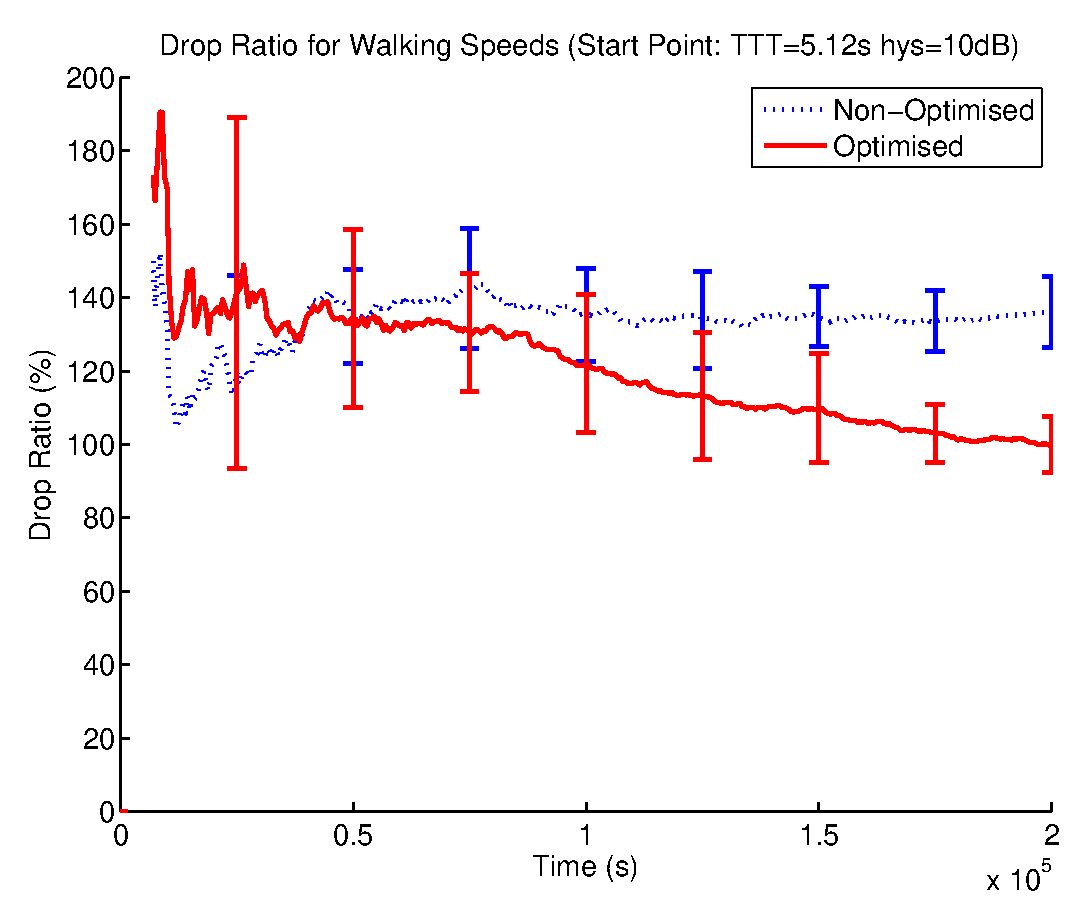
\includegraphics[width=0.66\textwidth]{figures/walking_figures/walkhigh.eps}
    \end{center}
    \caption{Graph of Optimised vs. Non-Optimised Results for Starting Point TTT=5.12s hys=10dB when UE traveling at walking speeds.}
    \label{fig:walk_high_drop}
\end{figure}
Figure~\ref{fig:walk_high_ttthys} shows how the TTT and hys values for base stations  5 and 8 optimised over a simulation run. It can be seen in Figure~\ref{fig:walk_high_ttt} that both base stations were in consensus to reduce the value of their TTT from the starting value of $5.12 s$. However, both base stations were not in consensus for how much the value should be reduce by. Base station 8 reduced its TTT value to as low as $0.16 s$ before settling between it and $0.256 s$. Base station 5 on the other hand reduced its TTT value a lot less, only going as low as to oscillate between $1.024 s$ and $1.28 s$. It can also be seen that Base station 5 oscillated a lot between those two values and this could be an indication that the algorithm had got stuck between two non-optimal states and was not able to optimise the value anymore. This means that even though the optimisation improved the performance there was a large window of potential for further improvement.
 
While both base station 5 and 8 were in consensus about reducing their TTT values, they were not in consensus about their hys values. It can be seen in Figure~\ref{fig:walk_high_hys} that base station 5 did not try to reduce its value of hys at all and only oscillated between, the starting value of, $10 dB$ and $9.5 dB$. This is a stark contrast to base station 8 which greatly reduced its value of hys as low as $5 dB$ before oscillating between it and $5.5 dB$. Again, much like with the TTT values, base station 5 appears to oscillate between two non-optimal values as the oscillations are quite frequent and the learning agent for that base station has not tried any other values to see if they give an improvement. Also since base station 8 reduce its value greatly before oscillating between two values could mean that it reached what it thinks to be an optimal state.
\begin{figure}[H]
        \centering
        \begin{subfigure}[b]{0.49\textwidth}
                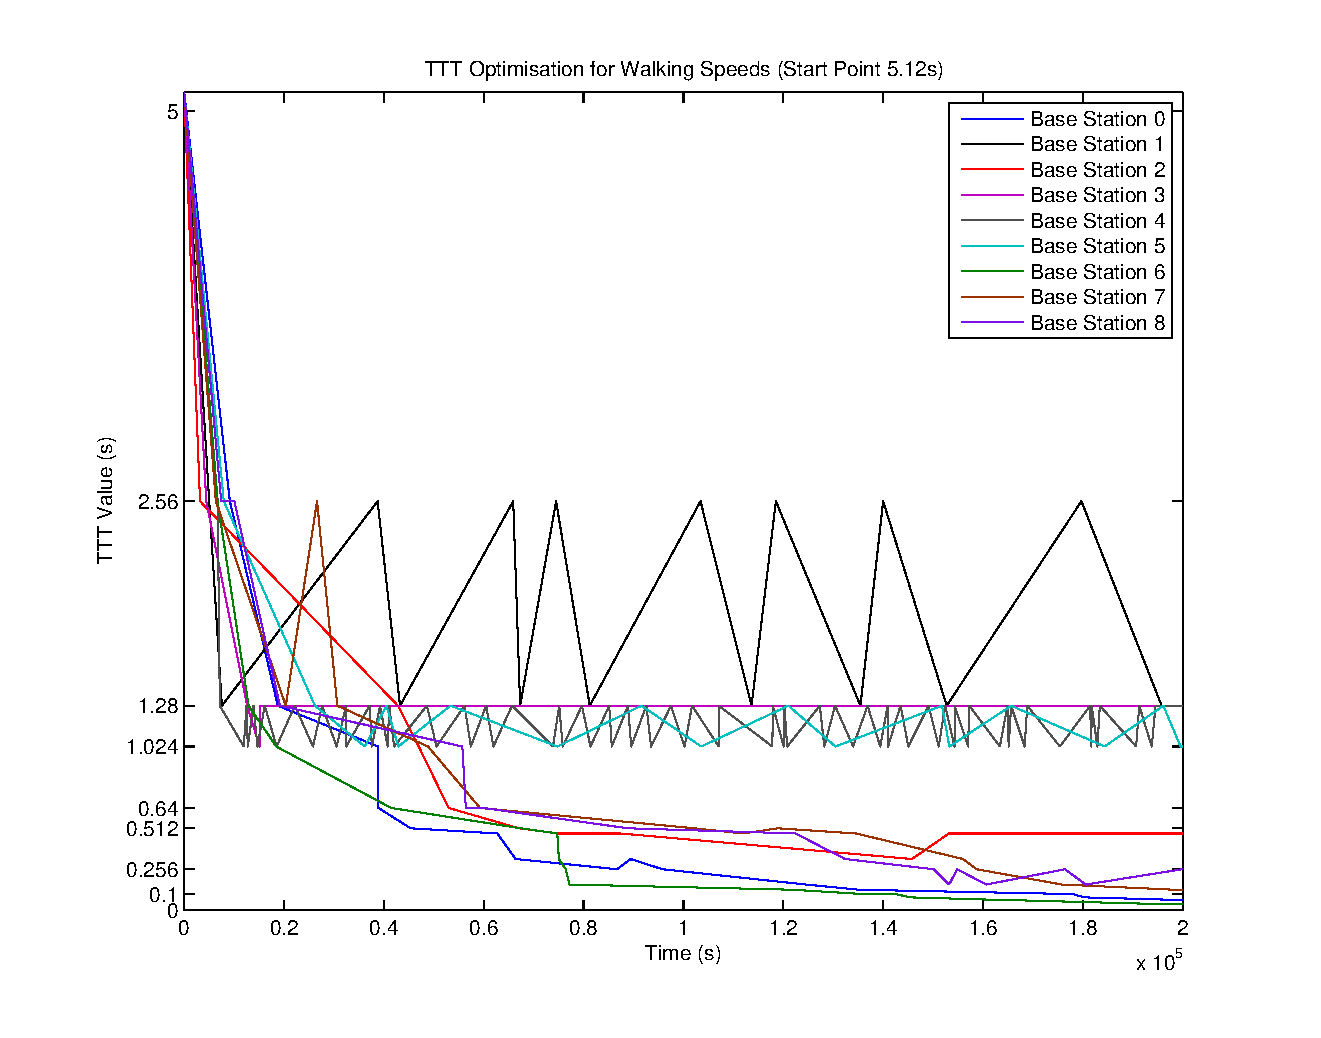
\includegraphics[width=\textwidth]{figures/walking_figures/high/long_ttt.eps}
                \caption{Changing TTT Values}
                \label{fig:walk_high_ttt}
        \end{subfigure}%
        ~ %add desired spacing between images, e. g. ~, \quad, \qquad etc.
          %(or a blank line to force the subfigure onto a new line)
        \begin{subfigure}[b]{0.49\textwidth}
                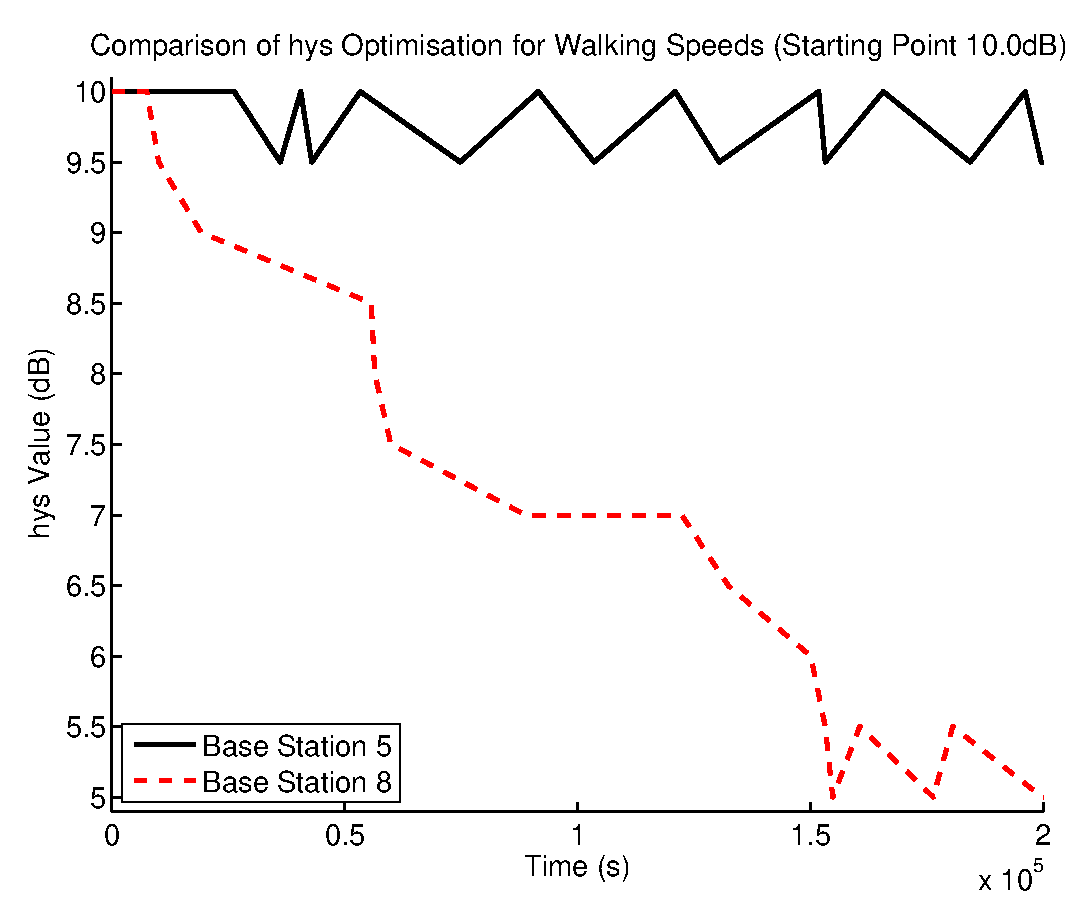
\includegraphics[width=\textwidth]{figures/walking_figures/high/long_hys.eps}
                \caption{Changing hys Values}
                \label{fig:walk_high_hys}
        \end{subfigure}
        \caption{Illustration of how the TTT and hys values changed over time for large values when UE traveling at walking speeds.}\label{fig:walk_high_ttthys}
\end{figure}
From these results it can be said that the system performed as expected by with the base stations shown having reduced both their values of TTT and hys. There were also a very high number for dropped calls and no ping-pong's, which was also expected in the simulation. All the graphs for the optimisation of the TTT and hys values for this scenario can be found in Appendix~\ref{ap:walk_large}.
\subsection{Middle Starting Values}
Again as seen in Figure~\ref{fig:walk_mid_drop} the optimisation process performed a lot better than the static values when they were originally set to the their middle values of 0.256 seconds for TTT and 5 dB for hys. The results also show that unlike with the results seen in Figure~\ref{fig:walk_high_drop} the optimisation process did not greatly increase the number of dropped call at first. Instead it was the non-optimised values that began with the large number of dropped calls. This means that when these dropped calls began to appear the machine learning algorithm changed the value of TTT and hys in such a way that the dropped calls seen for the non-optimised values did not happen.
\begin{figure}[H]
  \begin{center}
    	  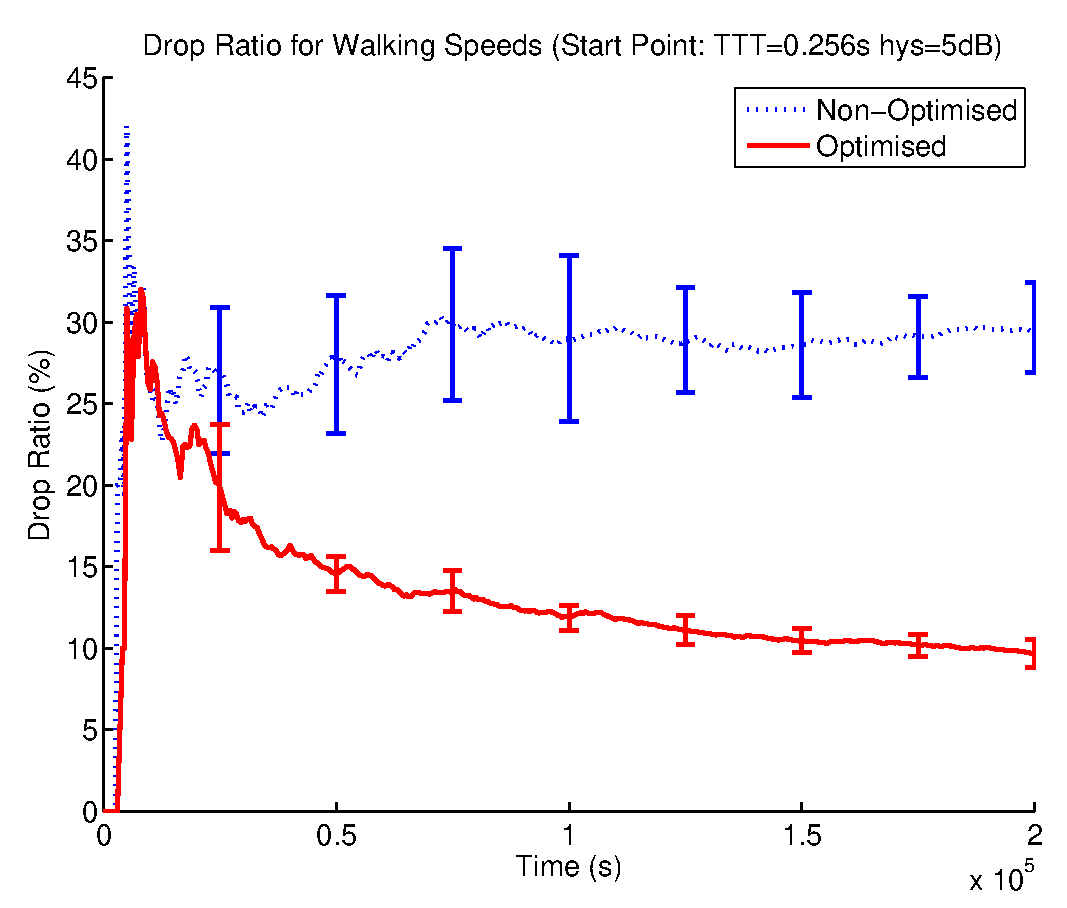
\includegraphics[width=0.75\textwidth]{figures/walking_figures/walkmid.eps}
    \end{center}
    \caption{Graph of Optimised vs. Non-Optimised Results for Starting Point TTT=0.256s hys=5dB when UE traveling at walking speeds.}
    \label{fig:walk_mid_drop}
\end{figure}
A comparison of how base stations 4 and 8 optimised their TTT and hys values can be seen in Figure~\ref{fig:walk_mid_ttthys}. It can be seen in that the two base station took different approaches when trying to optimise their TTT and hys values. Base station 4 can be seen to have increased its TTT value and decreased its hys value, while base station 8 decreased its TTT value and increased its hys value. When looking at Figure~\ref{fig:walk_mid_ttt} it can be seen that base station 4 increases its value of TTT to $0.48 s$ and then keeps that value steady. However, it can also be seen in Figure~\ref{fig:walk_mid_hys} that its value of hys actually ends up oscillating between $4 dB$ and $4.5 dB$ and oscillating quite frequently at first before settling at $4 dB$ for the last quarter of the simulation. Therefore, while the state of TTT being $0.48 s$ and hys being $4 dB$ may not have looked like an optimal state at first, the fact that it made no changes to any values for the last quarter of the simulation means that it could be a very optimal state for the base station.

It is interesting to see that base station 8 actually ended up oscillating between the same two states in both this scenario and the scenario seen in Section~\ref{walk_high}. With both of these scenarios finished between the same states of TTT equalling $0.16 s$, hys equalling $5 dB$ and TTT equalling $0.256 s$, hys equalling $5.5 dB$ it means that the learning agent for that base station managed to find what it thinks be an optimal set of states and end up there when starting at two different states, this is a very promising result. 
\begin{figure}[H]
        \centering
        \begin{subfigure}[b]{0.49\textwidth}
                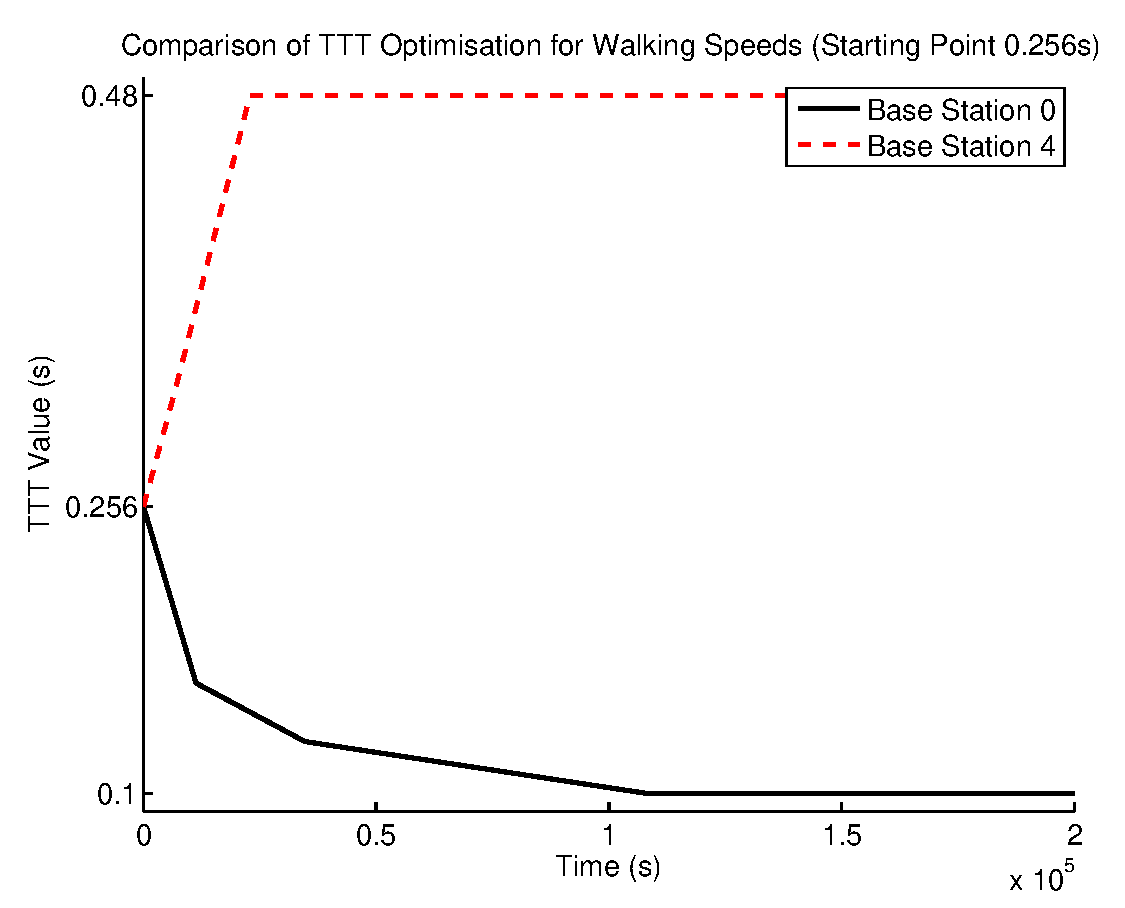
\includegraphics[width=\textwidth]{figures/walking_figures/mid/long_ttt.eps}
                \caption{Changing TTT Values}
                \label{fig:walk_mid_ttt}
        \end{subfigure}%
        ~ %add desired spacing between images, e. g. ~, \quad, \qquad etc.
          %(or a blank line to force the subfigure onto a new line)
        \begin{subfigure}[b]{0.49\textwidth}
                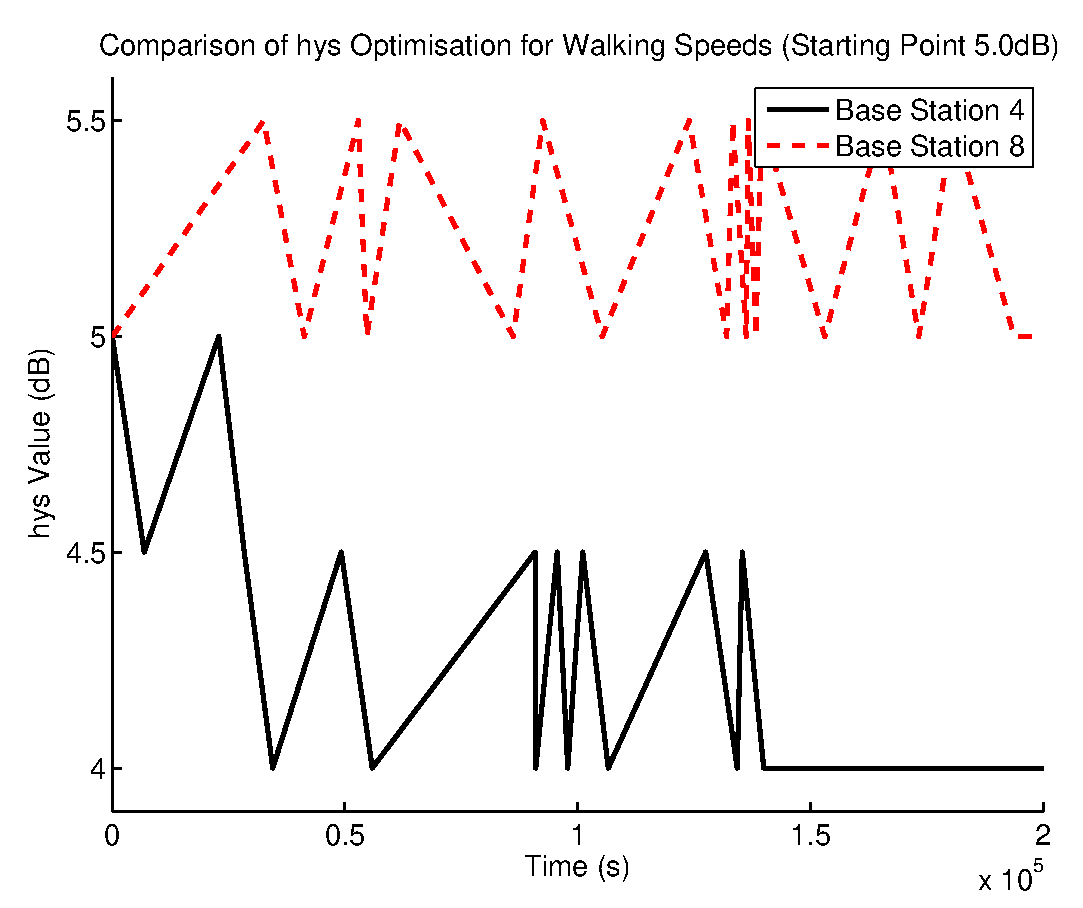
\includegraphics[width=\textwidth]{figures/walking_figures/mid/long_hys.eps}
                \caption{Changing hys Values}
                \label{fig:walk_mid_hys}
        \end{subfigure}
        \caption{Illustration of how the TTT and hys values changed over time for medium values when UE traveling at walking speeds.}\label{fig:walk_mid_ttthys}
\end{figure}
From the base stations compared above, while the performance was increased a lot, these two base stations did not optimised the values as expected. Instead of reducing both values they both opted for a split approach increased one value while decreasing the other. All the graphs for the optimisation of the TTT and hys values for this scenario can be found in Appendix~\ref{ap:walk_mid}.
\subsection{Small Starting Values}\label{sec:walk_low}
It turned out that ping-pong's were a very rare occurrence in the simulation. This was most likely due to there being no fading in the simulation and that Random Direction mobility model would having the UE moving in one direction for a long time meaning that the only likely occurrence of a ping-pong would be if a handover took place and the UE then turned around and moved the other direction.

Figure~\ref{fig:walk_low_ping} shows how the optimisation system performed against the static values when the simulation started with the TTT being 0 seconds and the hys being 0 dB. It can be seen that the optimisation process and the static values performed very similar. It can be seen though that the error bars for the optimised system become a lot smaller, than those for the static values, the longer the simulation is run. This means that the optimisation system would be expected to perform better the majority of the time.
\begin{figure}[H]
  \begin{center}
    	  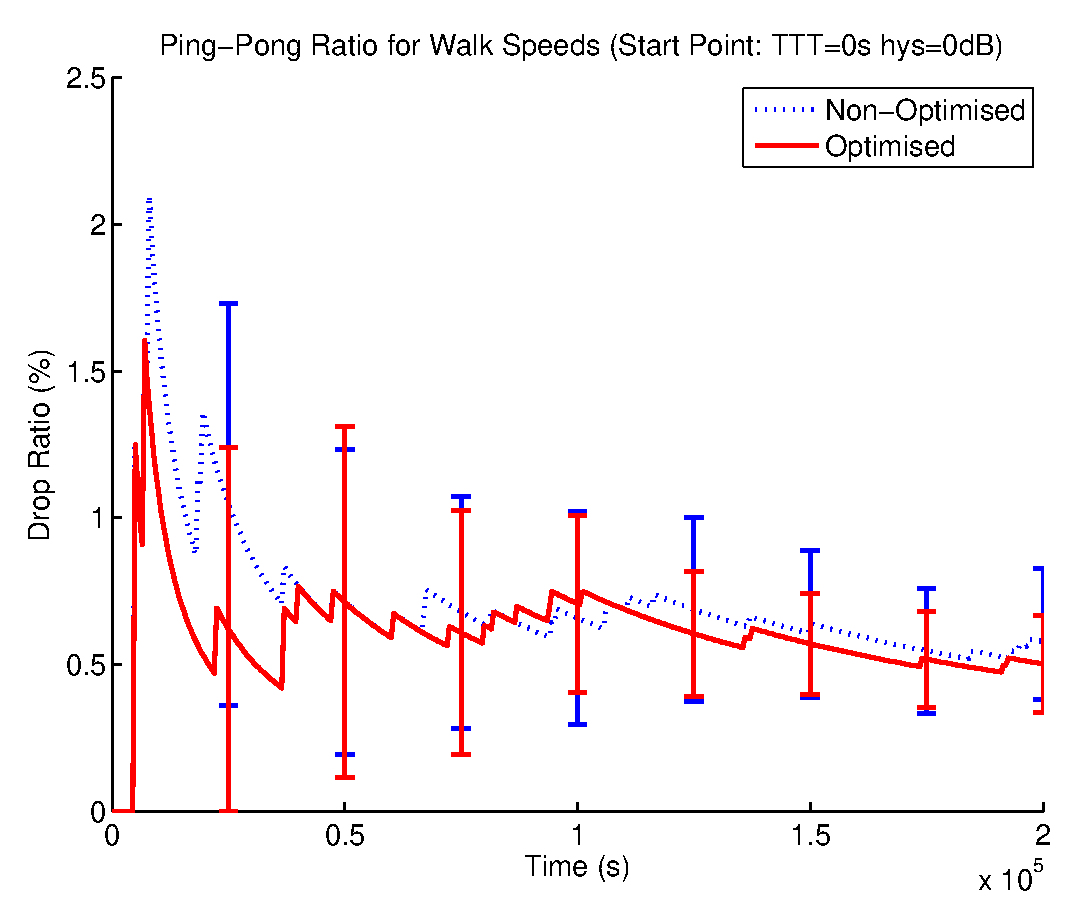
\includegraphics[width=0.75\textwidth]{figures/walking_figures/walklow.eps}
    \end{center}
    \caption{Graph of Optimised vs. Non-Optimised Results for Starting Point TTT=0s hys=0dB when UE traveling at walking speeds.}
    \label{fig:walk_low_ping}
\end{figure}
A comparison of how base stations 3 and 5 changed their values of TTT and hys when a ping-pong occurred can be seen in Figure~\ref{fig:walk_low_ttthys}. It can be seen that while both base stations only encounter one ping-pong each they both reacted differently when they occurred. It can be seen that base station 5 increased both its values of TTT and hys from $0 s$ and $0 dB$ to $0.04 s$ and $0.5 dB$ respectively.  Base station 3, however, decided to keep its value of TTT as $0 s$ and only increase its hys to $0.5 dB$. It is difficult to make any assumptions on which base station made the correct changes to their values as not a lot of changes actually happened.
\begin{figure}[H]
        \centering
        \begin{subfigure}[b]{0.49\textwidth}
                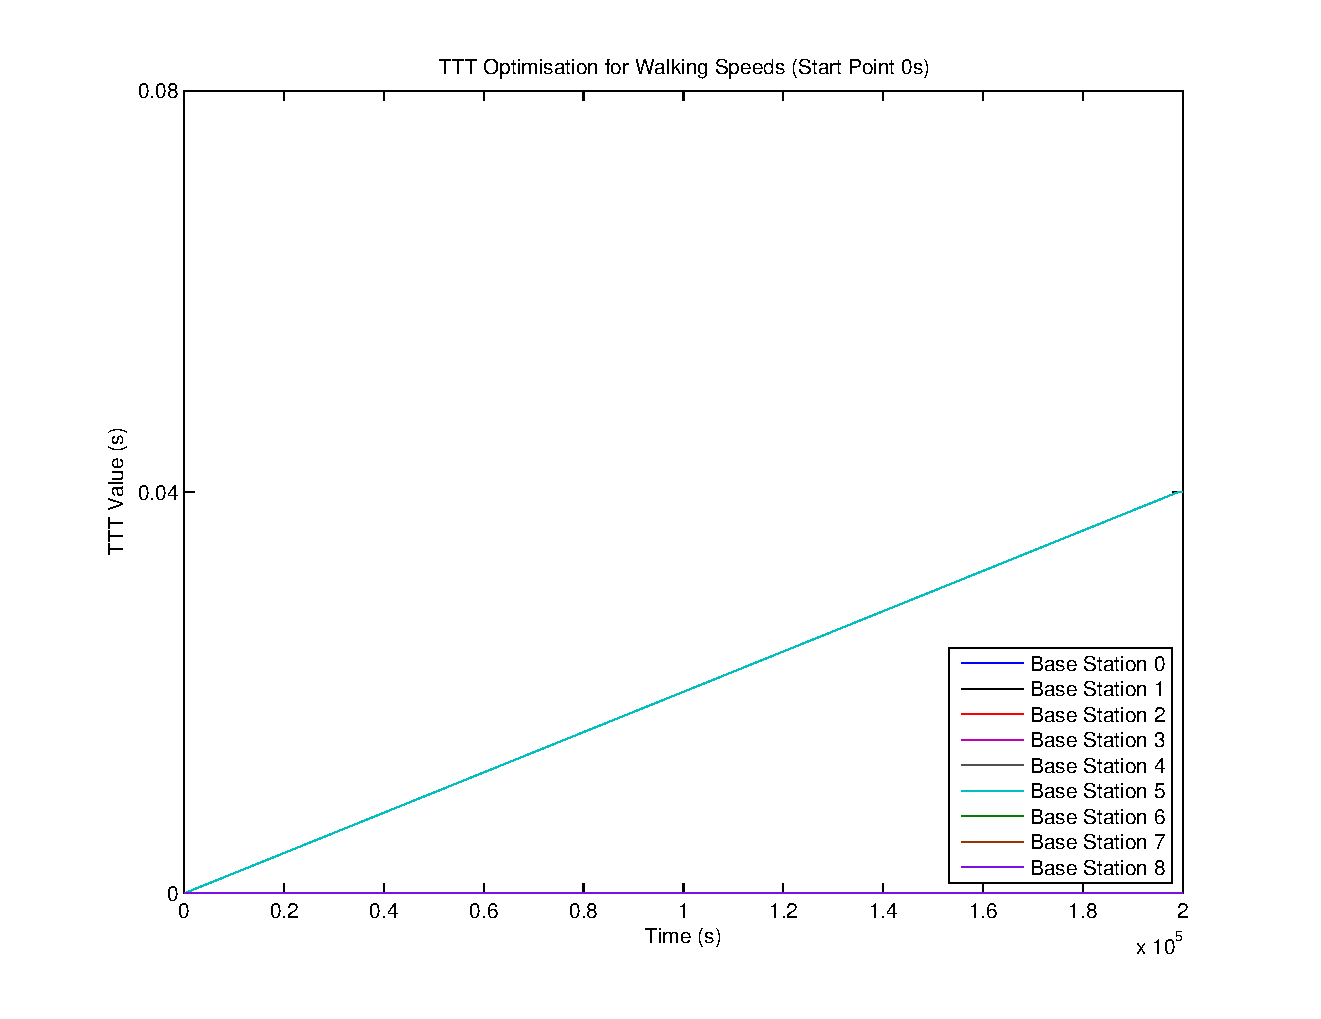
\includegraphics[width=\textwidth]{figures/walking_figures/low/long_ttt.eps}
                \caption{Changing TTT Values}
                \label{fig:walk_low_ttt}
        \end{subfigure}%
        ~ %add desired spacing between images, e. g. ~, \quad, \qquad etc.
          %(or a blank line to force the subfigure onto a new line)
        \begin{subfigure}[b]{0.49\textwidth}
                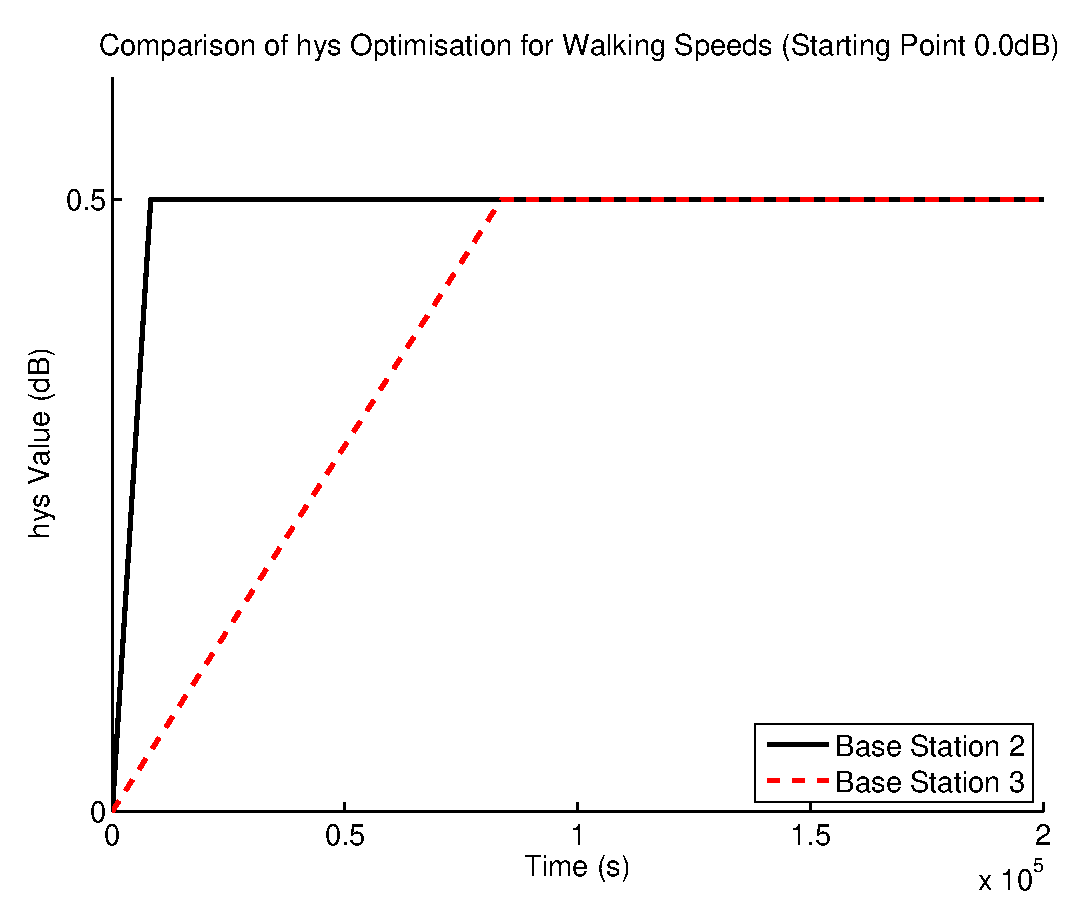
\includegraphics[width=\textwidth]{figures/walking_figures/low/long_hys.eps}
                \caption{Changing hys Values}
                \label{fig:walk_low_hys}
        \end{subfigure}
        \caption{Illustration of how the TTT and hys values changed over time for medium values when UE traveling at walking speeds.}\label{fig:walk_low_ttthys}
\end{figure}
This scenario played out as expected with no dropped calls occurring; instead having ping-pong’s determine the performance of the system. The system also compensated for this as expected by increase the values of TTT and hys as seen with base stations 3 and 5 and by the end of the simulation run the performance of the optimised values had become better than that of the non-optimised values. All the graphs for the optimisation of the TTT and hys values for this scenario can be found in Appendix~\ref{ap:walk_low}.
\subsection{Large hys and Small TTT Starting Values}
Much like the first three scenarios, it can be seen in Figure~\ref{fig:walk_highhys_drop} that, the optimisation system performed better than the static values when the TTT and hys started at 0.08 seconds and 7.5 dB respectively.
\begin{figure}[H]
  \begin{center}
    	  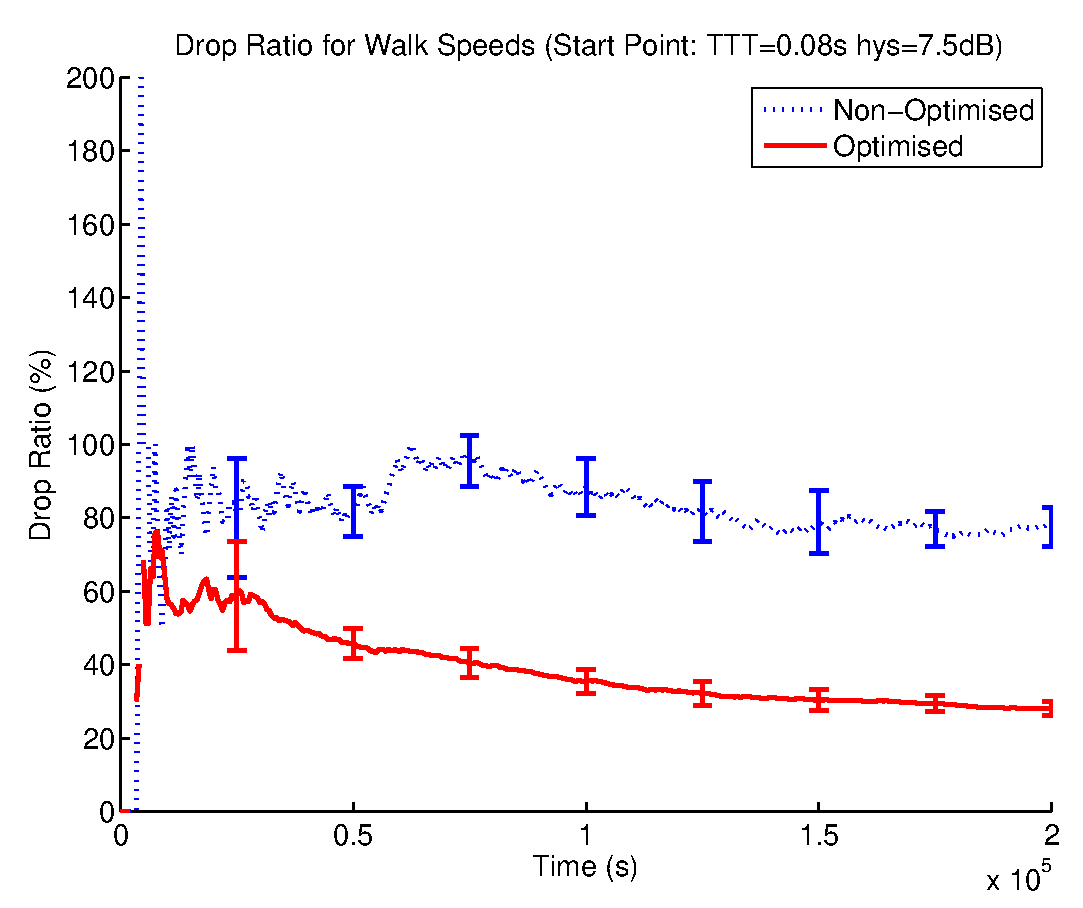
\includegraphics[width=0.75\textwidth]{figures/walking_figures/walkhighhys.eps}
    \end{center}
    \caption{Graph of Optimised vs. Non-Optimised Results for Starting Point TTT=0.08s hys=7.5dB when UE traveling at walking speeds.}
    \label{fig:walk_highhys_drop}
\end{figure}
A comparison of how base stations 4 and 7 attempted to optimised the system can be seen in Figure~\ref{fig:walk_highhys_ttthys}. It can be seen in Figure~\ref{fig:walk_highhys_ttt} that both base stations were in consensus to reduce the value slightly with both base stations oscillating between the starting value of $0.08 s$ and $0.064 s$ before they both became steady at $0.064 s$.

Figure~\ref{fig:walk_highhys_hys} shows that while both base stations were in consensus about their TTT values they were not in consensus about their hys values. It can be seen that base station 7 actually increased its value of hys and ended up oscillating between the starting value of $7.5 dB$ and $8 dB$. This is vastly different to the changes made by base station 4 which reduced the value all the way down to $3.5 dB$ and then stayed steady at that value.

It should also be noted that base station 4 appeared to reach an optimal state of TTT being $0.064 s$ and hys being $3.5 dB$ very quickly and stayed in this state for almost three quarters of the simulation run.
\begin{figure}[H]
        \centering
        \begin{subfigure}[b]{0.49\textwidth}
                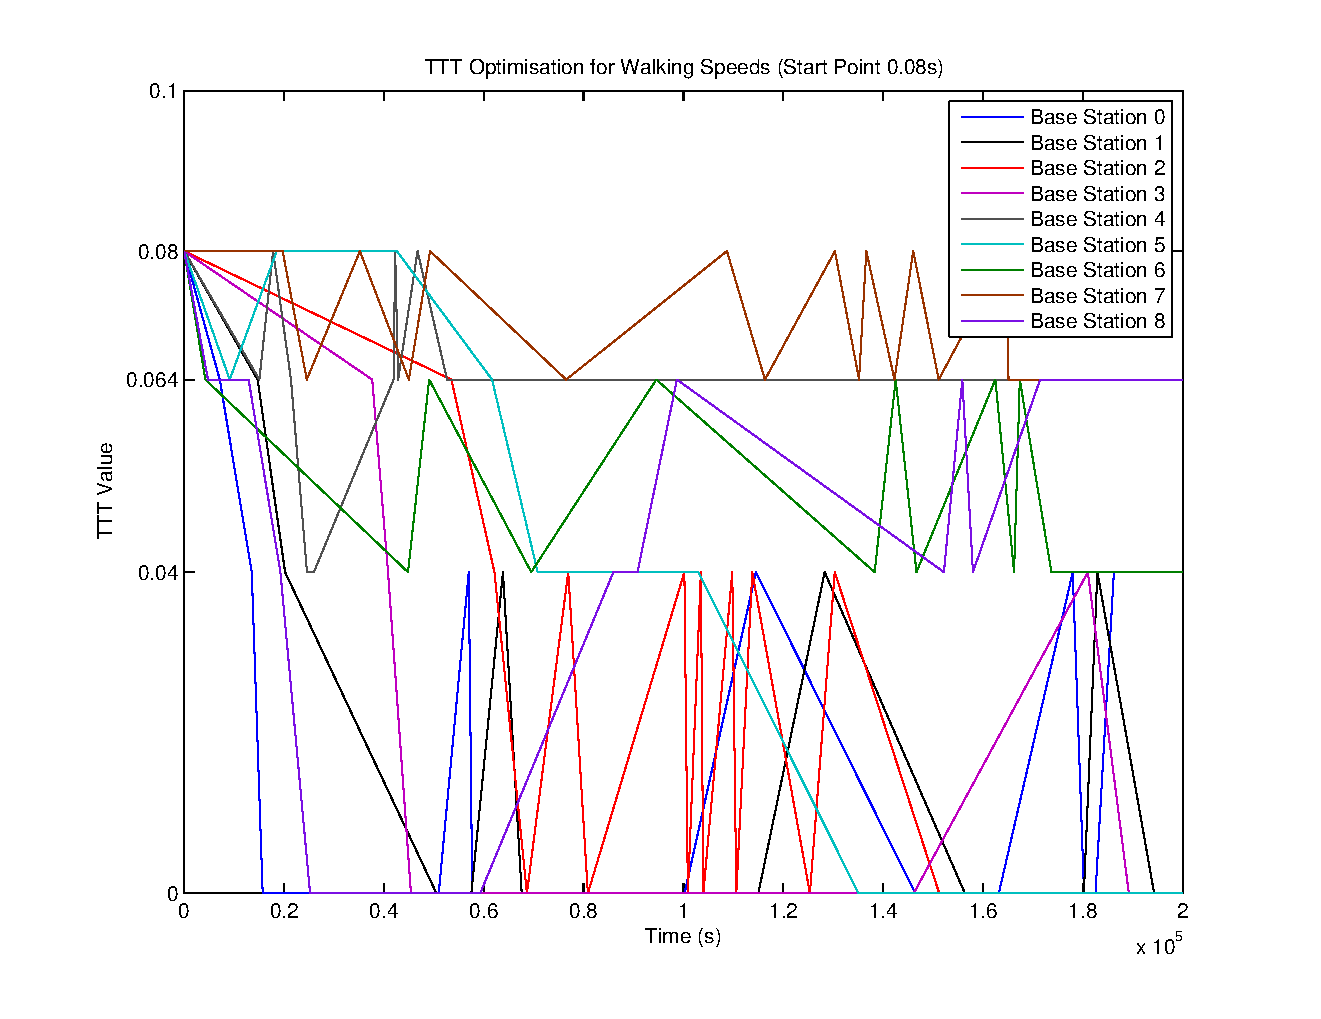
\includegraphics[width=\textwidth]{figures/walking_figures/highhys/long_ttt.eps}
                \caption{Changing TTT Values}
                \label{fig:walk_highhys_ttt}
        \end{subfigure}%
        ~ %add desired spacing between images, e. g. ~, \quad, \qquad etc.
          %(or a blank line to force the subfigure onto a new line)
        \begin{subfigure}[b]{0.49\textwidth}
                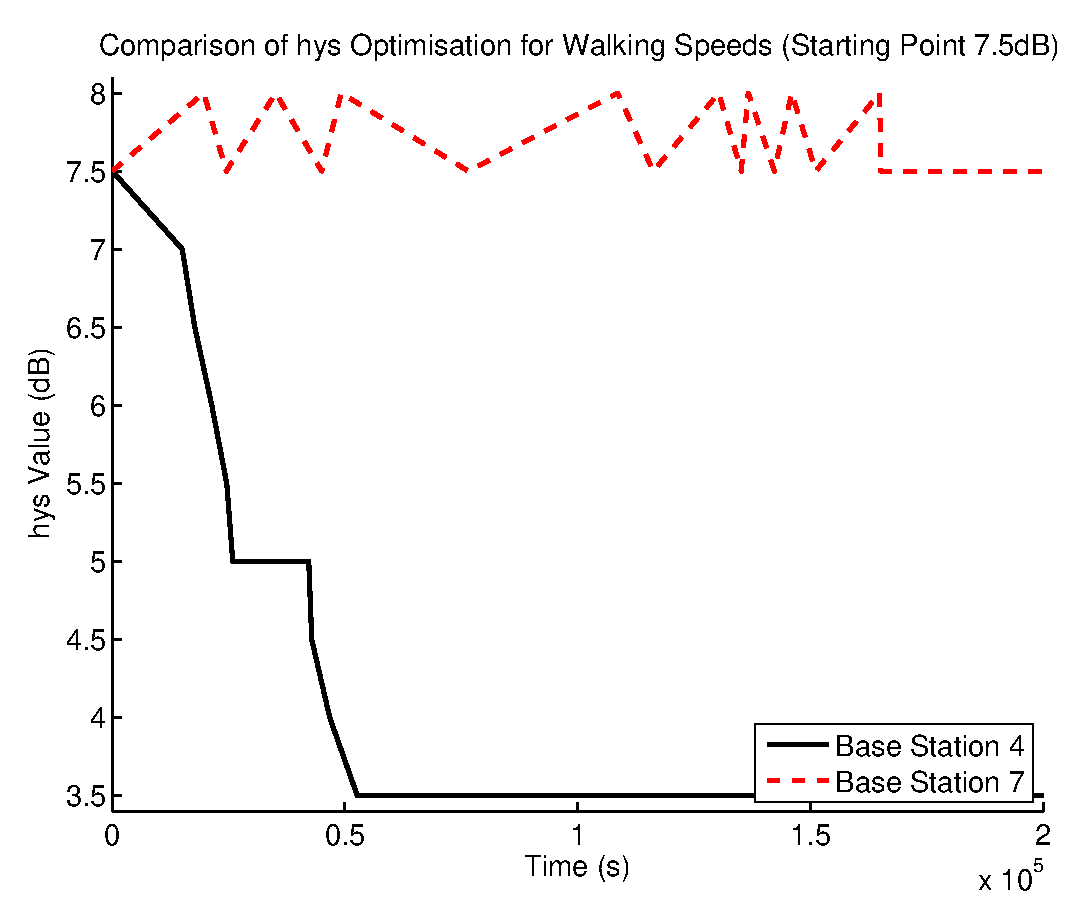
\includegraphics[width=\textwidth]{figures/walking_figures/highhys/long_hys.eps}
                \caption{Changing hys Values}
                \label{fig:walk_highhys_hys}
        \end{subfigure}
        \caption{Illustration of how the TTT and hys values changed over time for medium values when UE traveling at vehicle speeds.}\label{fig:walk_highhys_ttthys}
\end{figure}
In the comparison seen above the system did not perform entirely as expected.  While base station 4 did decrease its hys value, base station 7 actually increased it slightly, which was unexpected. Both base stations also performed expectantly decreasing their TTT values when they were expected to be increased. Even with this the system still performed better than the simulation when run with static values. All the graphs for the optimisation of the TTT and hys values for this scenario can be found in Appendix~\ref{ap:walk_highhys}.

\section{Vehicle Speed}\label{veh}
For the vehicle speed scenarios it is expected that number of dropped calls would increase over those seen in the walking speed scenarios due to the UE moving a lot faster and therefore giving a lot less time for the decision to handover or not. It is still expected that for the first scenario the system will reduce both values for TTT and hys. In the second scenario of the middle values it can also be expected the both values for TTT and hys will be reduced as dropped calls will still be expected fairly often at the speed the UE will be moving at. For the third scenario where both values for TTT and hys are at their lowest it is expected that the system will increase these values has ping-pong's should still be likely to happen, even at the high speeds. In the fourth scenario it is expected that the system is more likely to reduce both values, unlike when the UE was moving at walking speeds, because of the speed the UE is moving at decisions need to be made quickly.
\subsection{Large Starting Values}
It can be seen in Figure~\ref{fig:veh_high_drop} that the optimised system performed better than the system using the static values of 5.12 seconds for TTT and 10 dB for hys. 
\begin{figure}[H]
  \begin{center}
    	  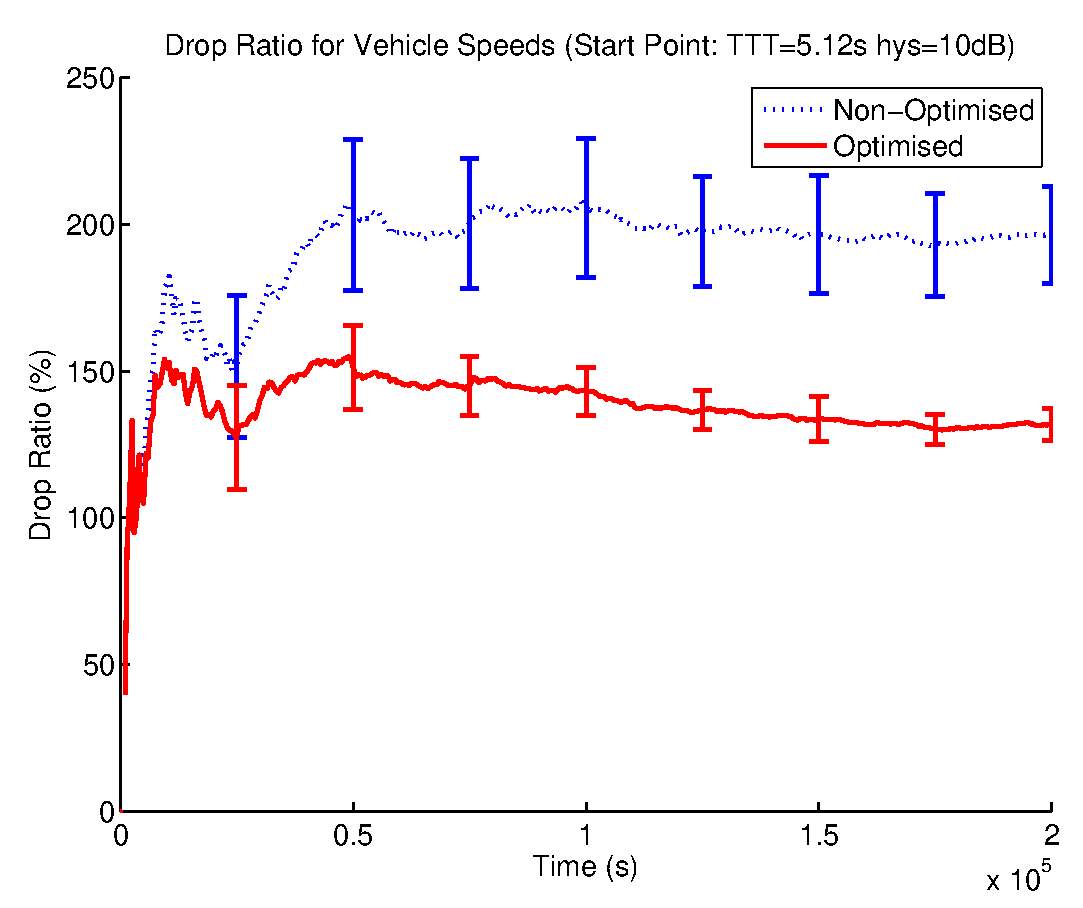
\includegraphics[width=0.75\textwidth]{figures/vehicle_figures/vehhigh.eps}
    \end{center}
    \caption{Graph of Optimised vs. Non-Optimised Results for Starting Point TTT=5.12s hys=10dB when UE traveling at walking speeds.}
    \label{fig:veh_high_drop}
\end{figure}
A comparison between how base stations 3 and 7 optimised their TTT and hys values can be seen in Figure~\ref{fig:veh_high_ttthys}. It can be seen in Figure~\ref{fig:veh_high_ttt} that both base stations were in consensus about what to do to their TT values which was to reduce them. However, both base stations were not in consensus about how much to reduce it by. Base station 3 reduced its value by only one single decrease to $2.56 s$ and then stayed steady at that value. Base station 7, however, reduced its value as low as $0.512 s$ before ending up oscillating between $1.024 s$ and $1.28 s$. the oscillation between those two values can be seen to be very frequent meaning the value should have been reduced more. This would make sense since the UE’s in this scenario are moving quickly meaning that there is less time for handovers to be triggered.

It can be seen in Figure~\ref{fig:veh_high_hys} that while base station 3 maybe have kept its value of TTT steady, its value of hys was oscillating extremely frequently between the starting value of $10 dB$ and $9.5 dB$. This means that those states are very likely non-optimal and the learning agent for the base station should have reduced that values a lot more. As for base station 7, it reduced its value of hys a lot more that base station 3 did and ended up oscillating between $6 dB$ and $6.5 dB$. Again the oscillation is very frequent and it is likely that the learning agent should have reduced the value more.
\begin{figure}[H]
        \centering
        \begin{subfigure}[b]{0.49\textwidth}
                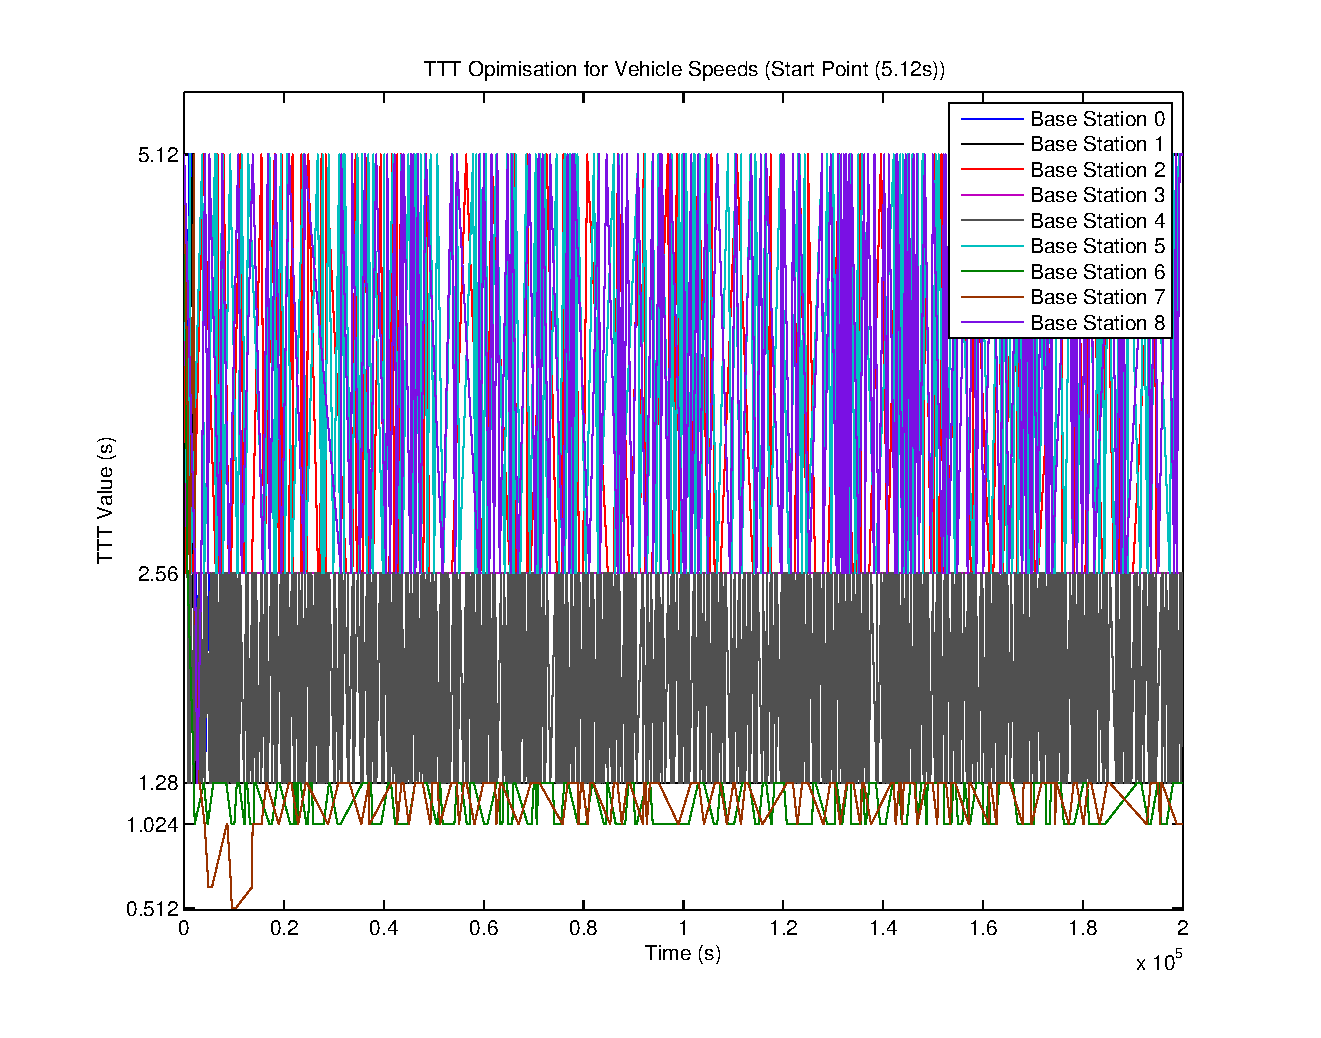
\includegraphics[width=\textwidth]{figures/vehicle_figures/high/long_ttt.eps}
                \caption{Changing TTT Values}
                \label{fig:veh_high_ttt}
        \end{subfigure}%
        ~ %add desired spacing between images, e. g. ~, \quad, \qquad etc.
          %(or a blank line to force the subfigure onto a new line)
        \begin{subfigure}[b]{0.49\textwidth}
                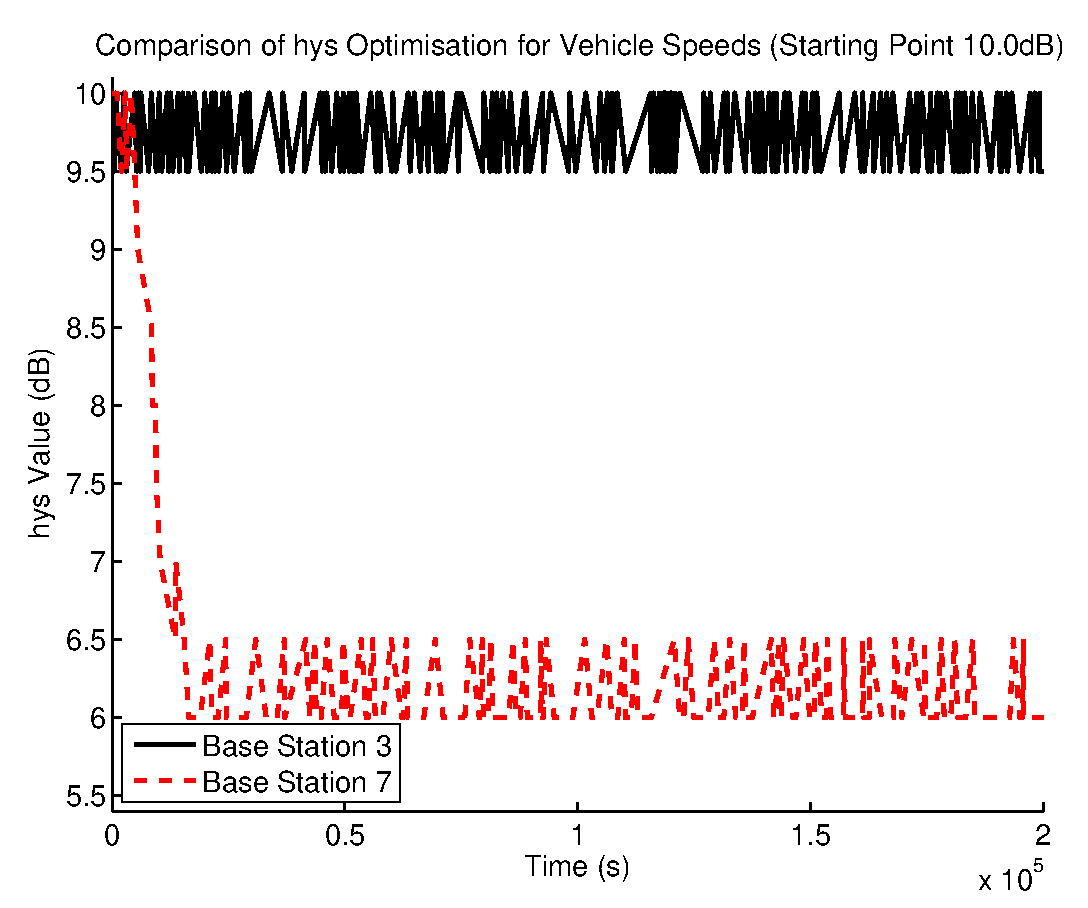
\includegraphics[width=\textwidth]{figures/vehicle_figures/high/long_hys.eps}
                \caption{Changing hys Values}
                \label{fig:veh_high_hys}
        \end{subfigure}
        \caption{Illustration of how the TTT and hys values changed over time for large values when UE traveling at vehicle speeds.}\label{fig:veh_high_ttthys}
\end{figure}
For this scenario while the system performed as expected and still performed better than that of the non-optimised system, it can be seen that it still did not perform all that well and appear be being getting stuck in non-optimal states. All the graphs for the optimisation of the TTT and hys values for this scenario can be found in Appendix~\ref{ap:veh_large}.
\subsection{Middle Starting Values}
In this scenario the optimised system perform much better than of the static values, where it TTT and hys values were initialised to 0.256 seconds and 5 dB respectively. The graphs of the dropped calls ratios can be seen in Figure~\ref{fig:veh_mid_drop}.
\begin{figure}[H]
  \begin{center}
    	  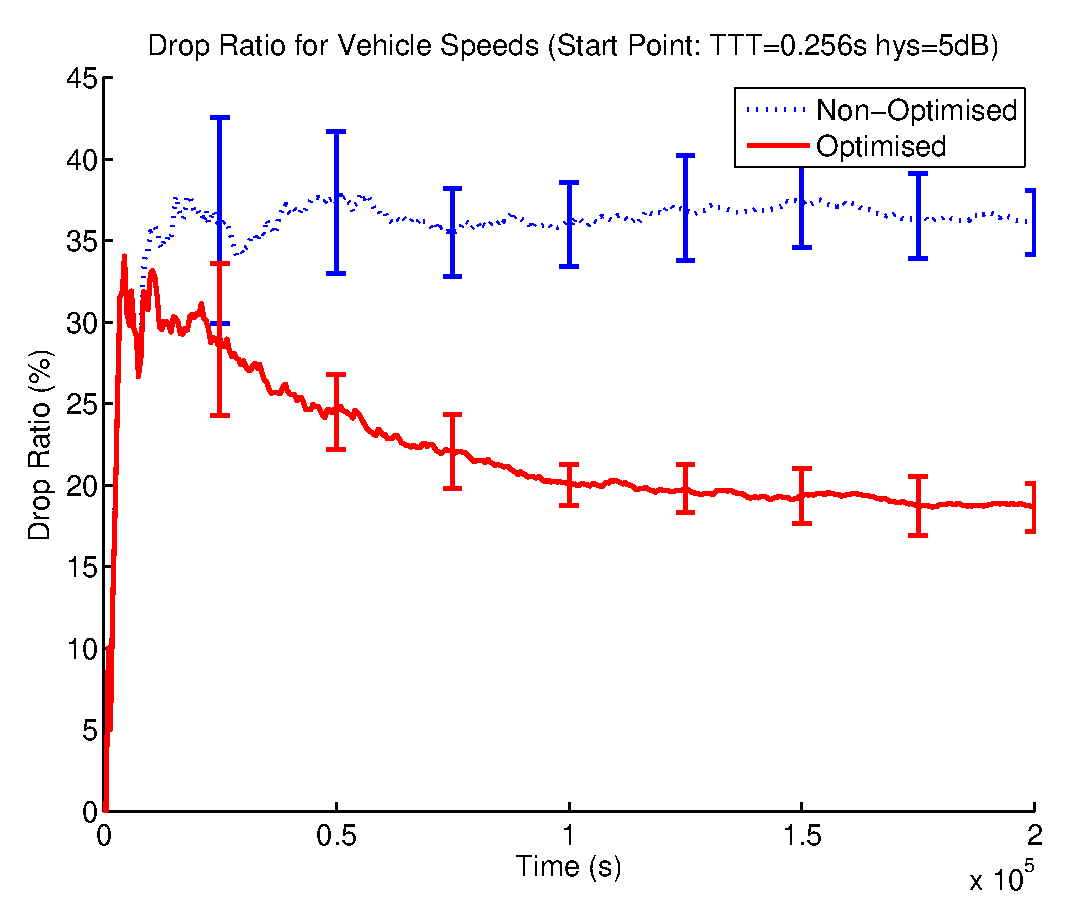
\includegraphics[width=0.75\textwidth]{figures/vehicle_figures/vehmid.eps}
    \end{center}
    \caption{Graph of Optimised vs. Non-Optimised Results for Starting Point TTT=0.256s hys=5dB when UE traveling at vehicle speeds.}
    \label{fig:veh_mid_drop}
\end{figure}
Figure~\ref{fig:veh_mid_ttthys} shows a comparison of how base stations 5 and 6 attempted to optimised their values of TTT and hys. It can be seen in Figure~\ref{fig:veh_mid_ttt} that the two base stations took completely different approaches to optimising their TTT values. Base station 5 reduced its value of TTT and actually ended up looping between $0.08 s$, $0.1 s$ and $0.128 s$, with the frequency of the changes being fairly frequent. Base station 6, however, increased its value of TTT as high as $1.28 s$ and ended up oscillating between that value and $1.024 s$, with its movements being slightly more frequent that those of base station 5. It is difficult to say which base station may be correct since both still made changes frequently while in oscillation, but since the UE’s are moving very fast in this scenario is would be assumed that base station 5’s made changes would be more correct.

Unlike with the changes base stations 5 and 6 made to their TTT values, they were in consensus about what changes should be made to their hys values. Both base stations end up oscillating between the starting value of $5 dB$ and $4.5 dB$.
\begin{figure}[H]
        \centering
        \begin{subfigure}[b]{0.49\textwidth}
                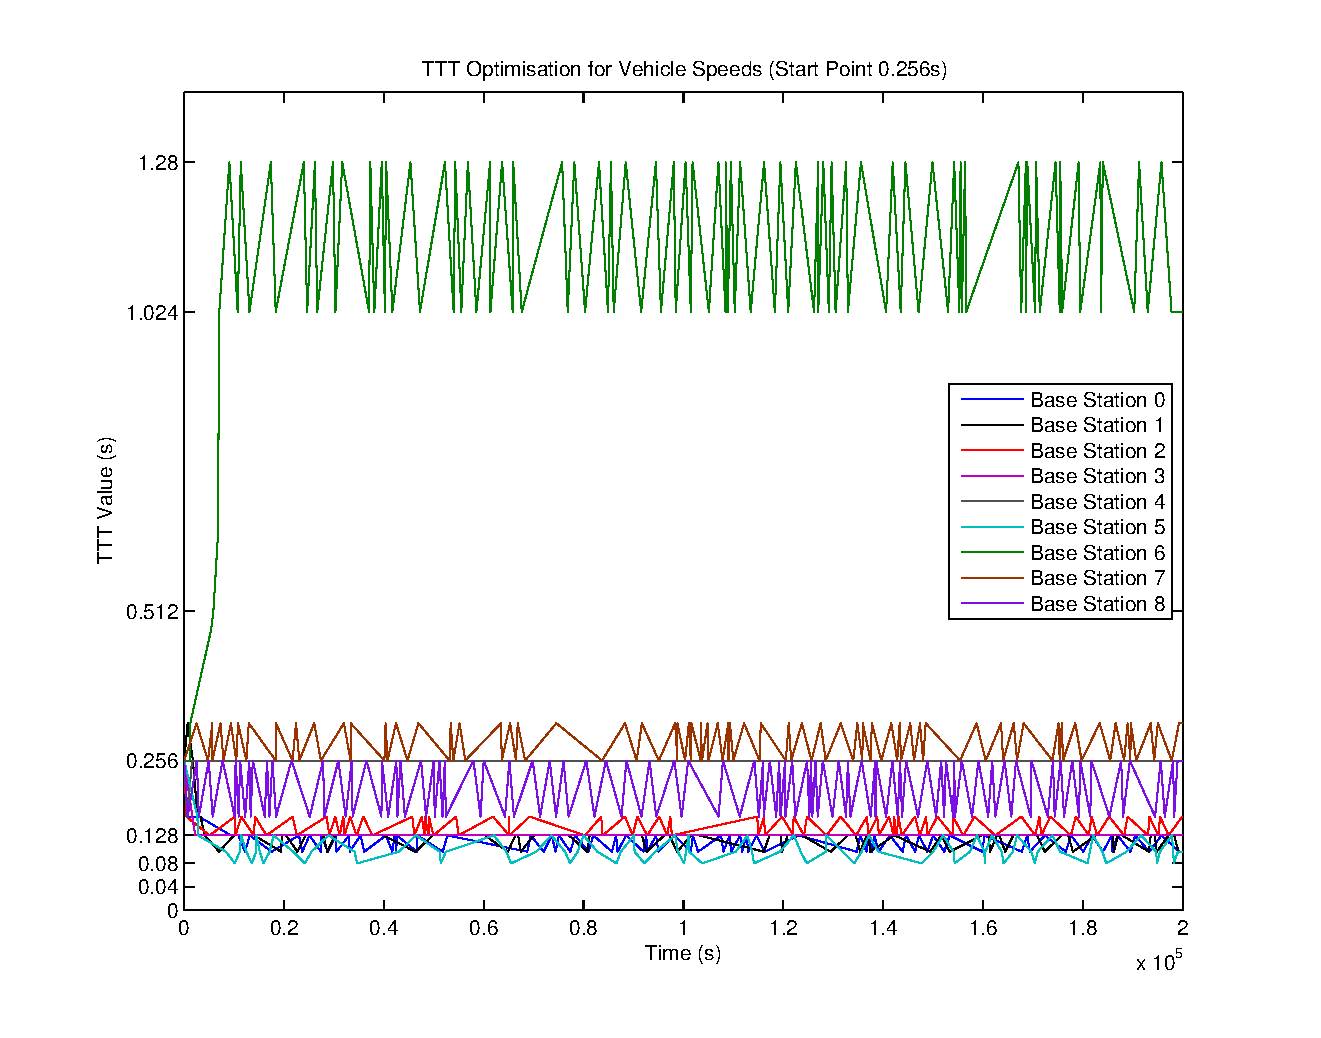
\includegraphics[width=\textwidth]{figures/vehicle_figures/mid/long_ttt.eps}
                \caption{Changing TTT Values}
                \label{fig:veh_mid_ttt}
        \end{subfigure}%
        ~ %add desired spacing between images, e. g. ~, \quad, \qquad etc.
          %(or a blank line to force the subfigure onto a new line)
        \begin{subfigure}[b]{0.49\textwidth}
                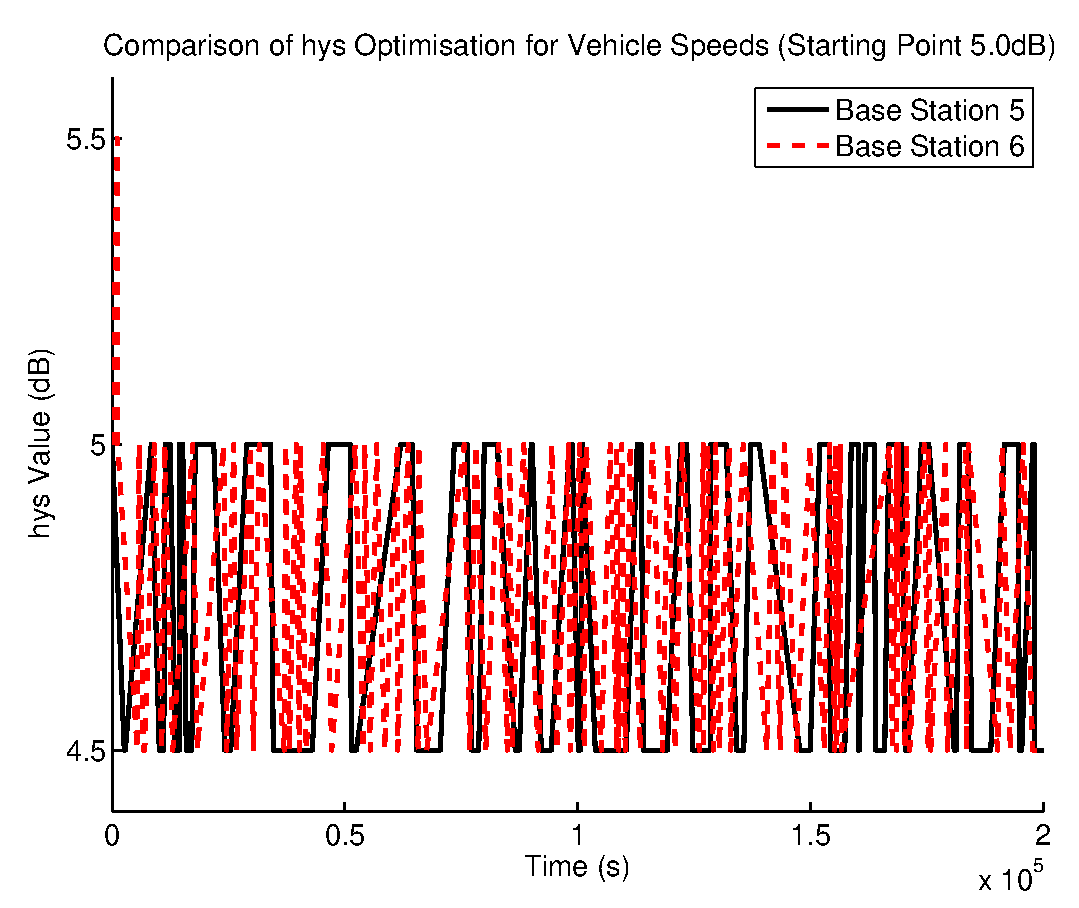
\includegraphics[width=\textwidth]{figures/vehicle_figures/mid/long_hys.eps}
                \caption{Changing hys Values}
                \label{fig:veh_mid_hys}
        \end{subfigure}
        \caption{Illustration of how the TTT and hys values changed over time for medium values when UE traveling at vehicle speeds.}\label{fig:veh_mid_ttthys}
\end{figure}
In this scenario it has been seen that base station 5 functioned as expected reducing both its values of TTT and hys. On the other hand base station 6 made very unexpected changes to its TTT value by actually greatly increasing its value. All the graphs for the optimisation of the TTT and hys values for this scenario can be found in Appendix~\ref{ap:veh_mid}.
\subsection{Small Starting Values}
It can be seen that for this scenario the optimised system and static values performed identically at first, but by the end the ratio of ping-pong's was better for the optimised system than that of the non-optimised values.
\begin{figure}[H]
  \begin{center}
    	  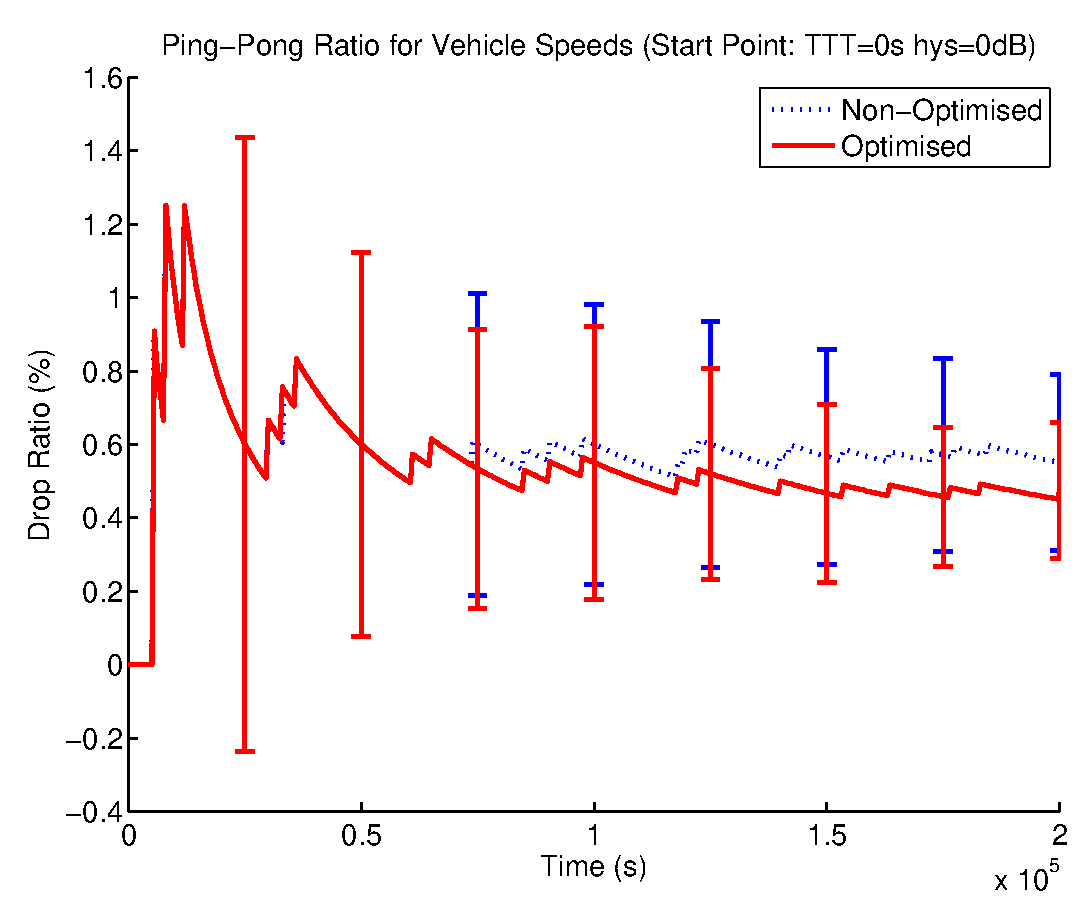
\includegraphics[width=0.75\textwidth]{figures/vehicle_figures/vehlow.eps}
    \end{center}
    \caption{Graph of Optimised vs. Non-Optimised Results for Starting Point TTT=0s hys=0dB when UE traveling at vehicle speeds.}
    \label{fig:veh_low_drop}
\end{figure}
Figure~\ref{fig:veh_low_ttthys} shows a comparison of how base stations 0 and 3 reacted when they experienced connection ping-pong’s. It can be seen that base station 3 actually encountered two ping-pong’s during this simulation run. It actually increased is TTT value after the first ping-pong to $0.04 s$ but after the second it actually reduced it back down to $0 s$. However, the learning agent for the base station increased its value of hys both times it encountered a ping-pong reaching $1 dB$ by the end of the simulation.

Unlike base station 3, base station 0 only encountered one ping-pong and it increased both its values of TTT and hys to $0.04 s$ and $0.5 dB$ respectively. Much like the results seen for this scenario when done with walking speeds it is hard to determined which base station made the correct changes as very few changes were actually made.
\begin{figure}[H]
        \centering
        \begin{subfigure}[b]{0.49\textwidth}
                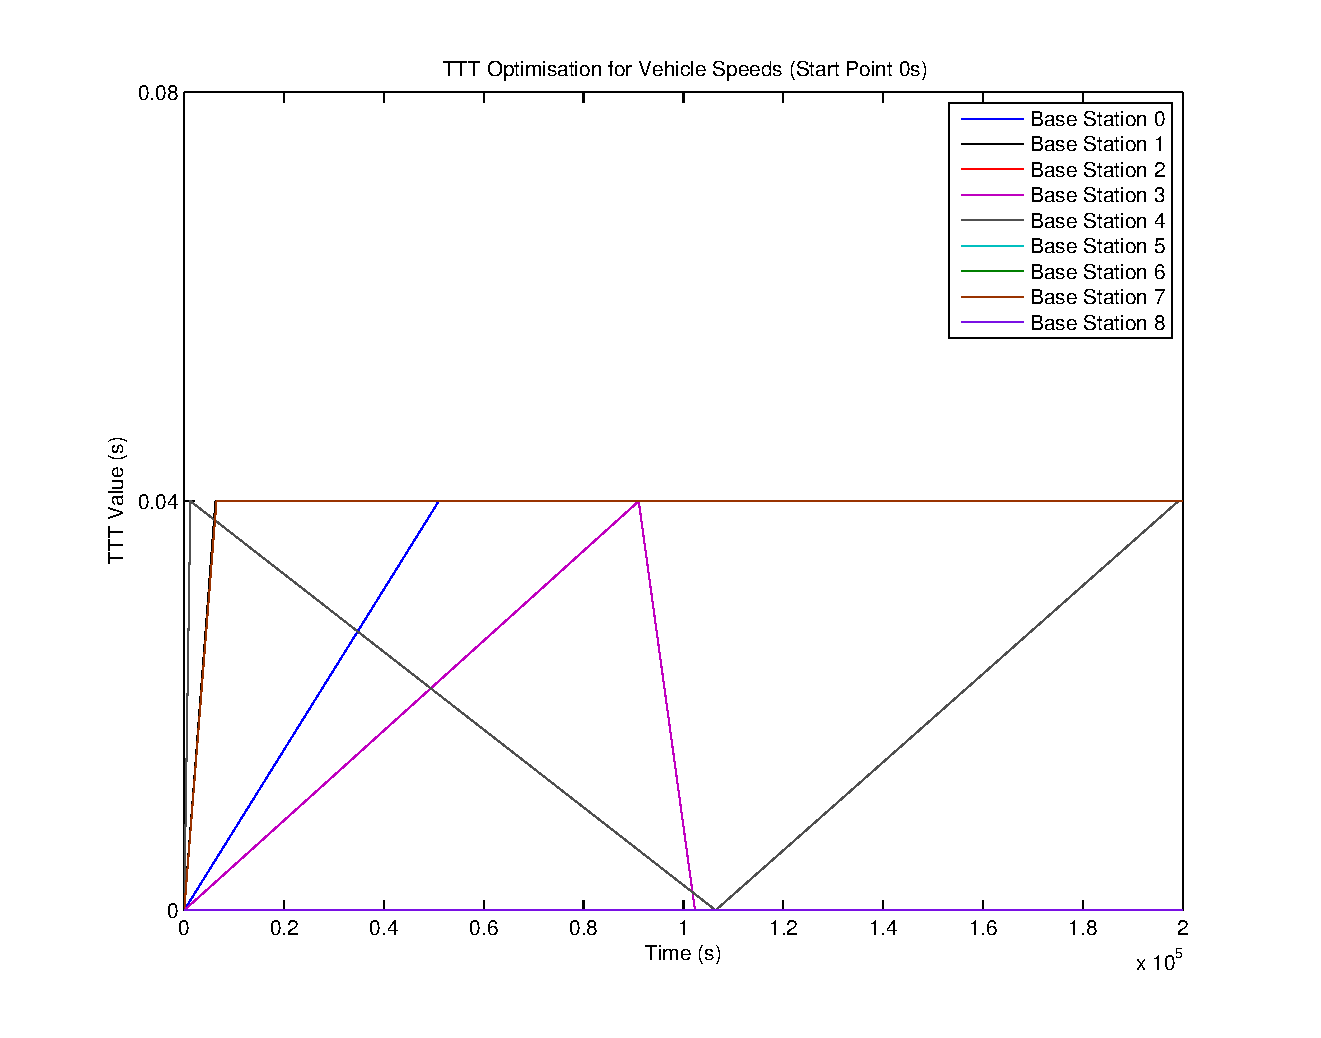
\includegraphics[width=\textwidth]{figures/vehicle_figures/low/long_ttt.eps}
                \caption{Changing TTT Values}
                \label{fig:veh_low_ttt}
        \end{subfigure}%
        ~ %add desired spacing between images, e. g. ~, \quad, \qquad etc.
          %(or a blank line to force the subfigure onto a new line)
        \begin{subfigure}[b]{0.49\textwidth}
                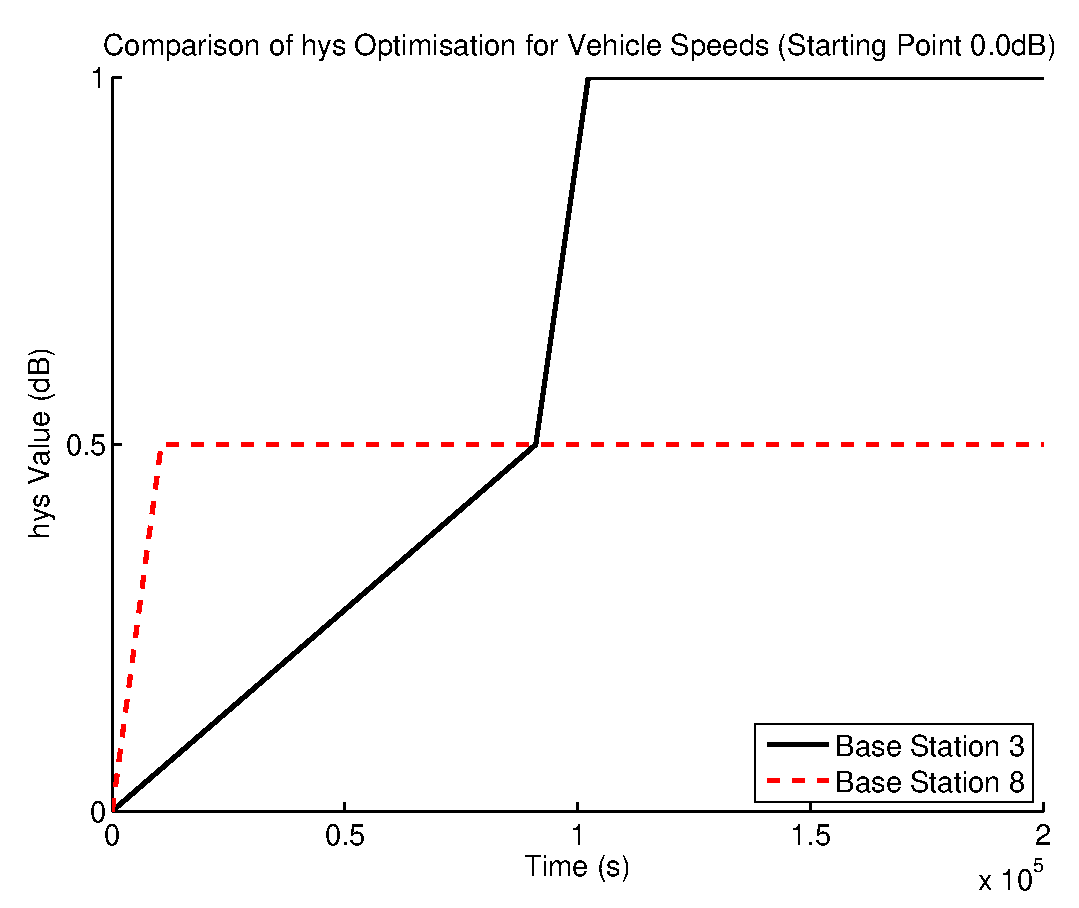
\includegraphics[width=\textwidth]{figures/vehicle_figures/low/long_hys.eps}
                \caption{Changing hys Values}
                \label{fig:veh_low_hys}
        \end{subfigure}
        \caption{Illustration of how the TTT and hys values changed over time for medium values when UE traveling at vehicle speeds.}\label{fig:veh_low_ttthys}
\end{figure}
Again the optimisation system functioned as expected with increasing both the TTT and hys values due to ping-pong's occurring. This was expected because even though the UE is travel quickly the system still has to make sure that it does not trigger a handover too quickly. All the graphs for the optimisation of the TTT and hys values for this scenario can be found in Appendix~\ref{ap:veh_low}.
\subsection{Large hys and Small TTT Starting Values}
As seen in the first three scenarios for the vehicle speed testing the optimised system managed to perform better than that of the non-optimised system when starting with the TTT being 0.08 seconds and the hys 7.5 dB. However, the improvement was not quite as great as seen in the other scenarios. 
\begin{figure}[H]
  \begin{center}
    	  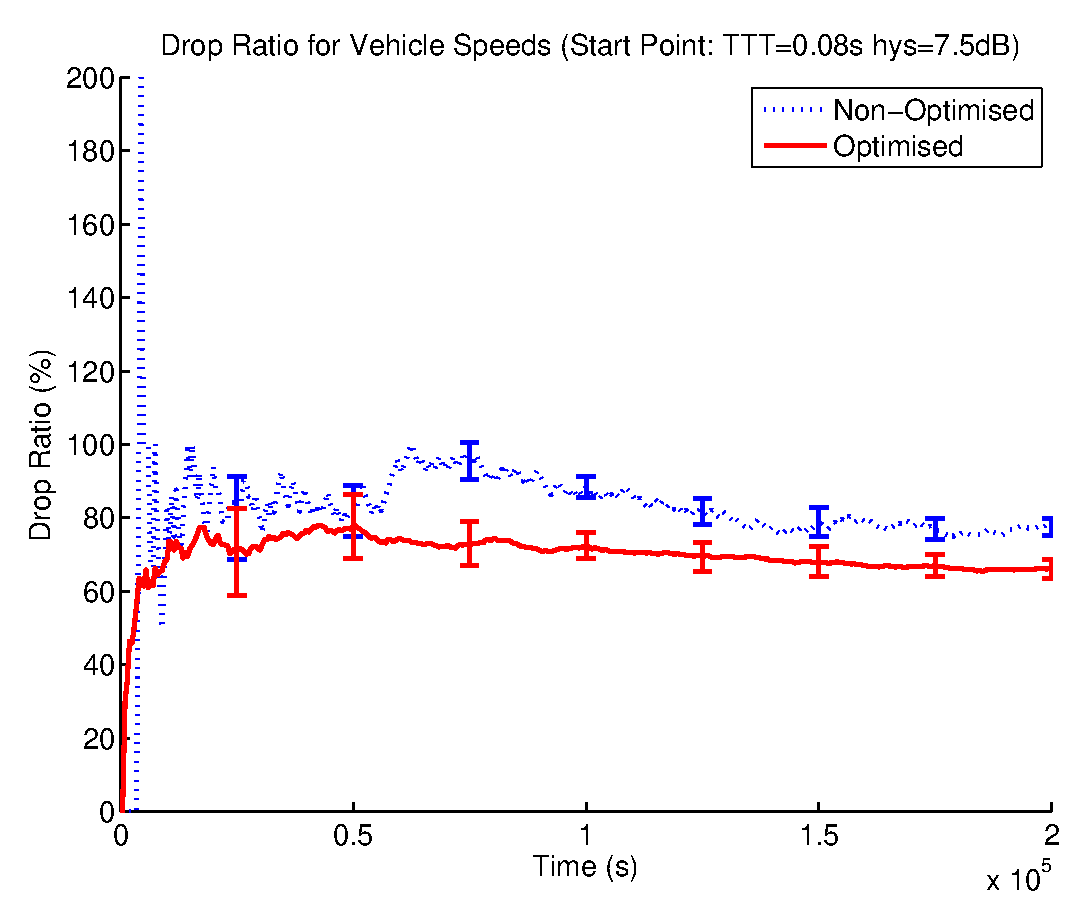
\includegraphics[width=0.75\textwidth]{figures/vehicle_figures/vehhighhys.eps}
    \end{center}
    \caption{Graph of Optimised vs. Non-Optimised Results for Starting Point TTT=0.08s hys=7.5dB when UE traveling at vehicle speeds.}
    \label{fig:veh_highhys_drop}
\end{figure}
A comparison of how base stations 0 and 5 attempted to optimise their TTT and hys values can be seen in Figure~\ref{fig:veh_highhys_ttthys}. It can be seen that base stations 0 and 5 both took different approaches to trying to optimise values of TTT and hys. Base station 0 reduced both its values of TTT and hys end up oscillating between $0 s$ and $0.04 s$ for TTT and $4.5 dB$ and $5 dB$ for hys. The oscillations were still fairly frequent meaning that there could have been more of an improvement.

Unlike base station 0, base station 5 actually increased both its values of TTT and hys, which was highly unexpected. The base station ended up oscillating between $0.08 s$ and $0.1 s$ for TTT and $8 dB$ and $8.5 dB$ for hys. Due to the speeds that the UE’s are moving at it could be said that these changes are wrong because due to the speed of the UE’s the handovers need to be triggered quickly and increasing the values from their starting points in this scenario would not do that.
\begin{figure}[H]
        \centering
        \begin{subfigure}[b]{0.49\textwidth}
                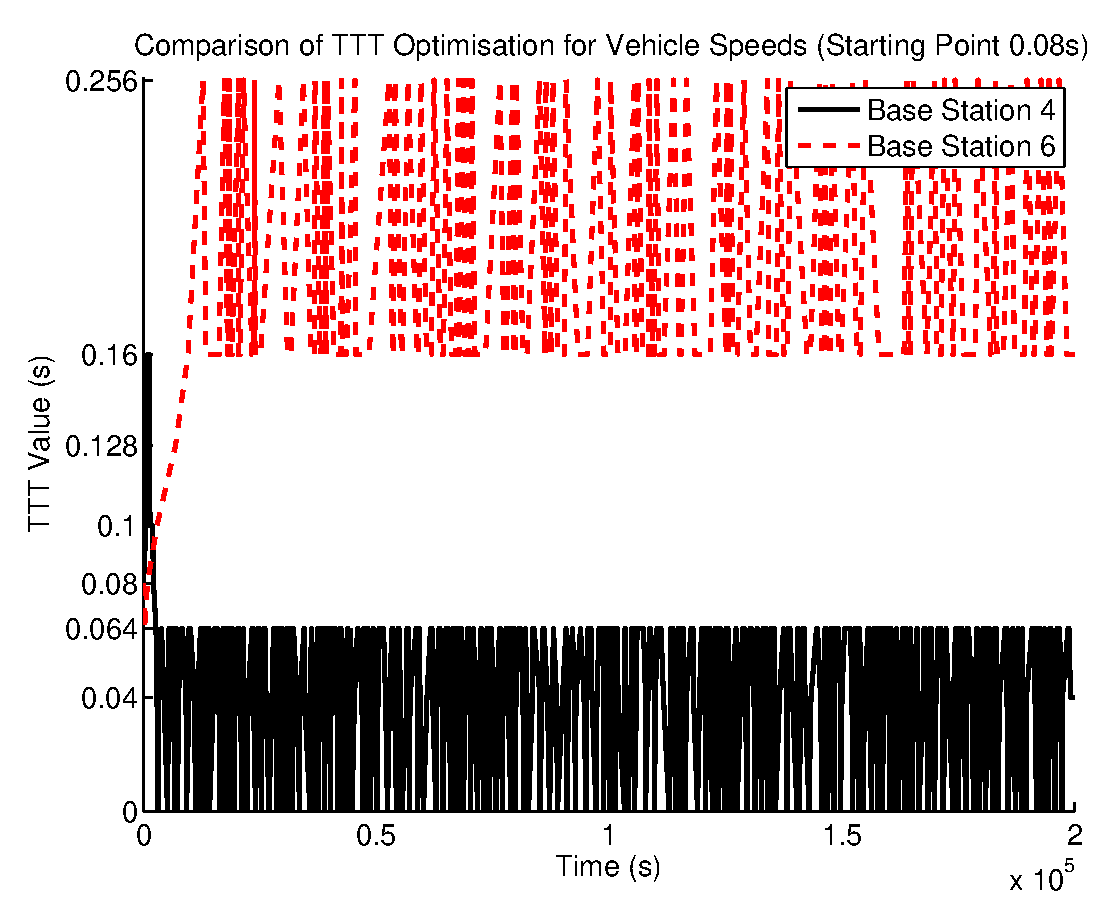
\includegraphics[width=\textwidth]{figures/vehicle_figures/highhys/long_ttt.eps}
                \caption{Changing TTT Values}
                \label{fig:veh_highhys_ttt}
        \end{subfigure}%
        ~ %add desired spacing between images, e. g. ~, \quad, \qquad etc.
          %(or a blank line to force the subfigure onto a new line)
        \begin{subfigure}[b]{0.49\textwidth}
                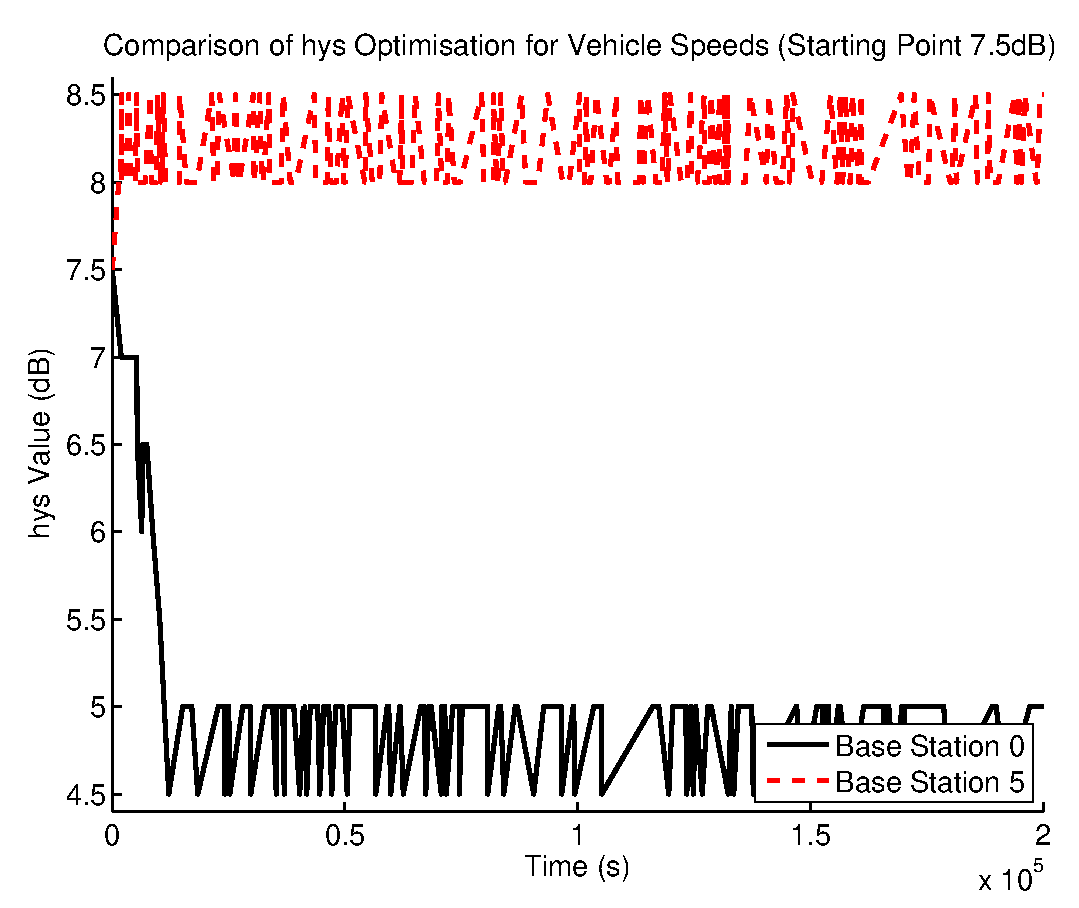
\includegraphics[width=\textwidth]{figures/vehicle_figures/highhys/long_hys.eps}
                \caption{Changing hys Values}
                \label{fig:veh_highhys_hys}
        \end{subfigure}
        \caption{Illustration of how the TTT and hys values changed over time for medium values when UE traveling at vehicle speeds.}\label{fig:veh_highhys_ttthys}
\end{figure}
Much like with the other scenarios it is seen that while the system may have been an improvement over the static values the system still could have performed far better, as base stations appeared to keep switching between values that could be considered non-optimal. All the graphs for the optimisation of the TTT and hys values for this scenario can be found in Appendix~\ref{ap:veh_highhys}.
\section{Evaluation}
Over the four scenarios used to test the optimisation system for walking speeds it can be seen that overall the system performed better than if no optimisation was done at all. It can also be seen that the system makes improvements to the performance very quickly. As seen in scenarios for the middle values and the large hys with small TTT the system managed to not have the large spike in dropped calls at the beginning of their simulation runs which were seen in there respective non-optimised runs.

In the scenarios for vehicle speeds it was seen that the system did performed better than if no optimisation was used. However, it was seen in the ways that the TTT and hys values were changed that they did not stop dropped calls constantly happening, which means that these values were likely non-optimal. Therefore it is possible that the system could have performed a lot better if the system did not get stuck between non-optimal states.

It can, however, be seen that when the system does not get stuck between non-optimal states that it will optimise the TTT and hys values as quickly as it is needed, i.e., whenever a dropped call or ping-pong occurs.

The optimisation system, however, also appears to have some drawbacks. It was seen in the first scenario that the optimisation system caused a very large increase to the dropped call ratio before improving it. This is a usual downside in optimisation processes where 'things have to get worse before they can get better' and this process is a part of Q-Learning where the possible future rewards are taken into account when selecting a new state to move to. It was also seen in the scenarios using the vehicle speeds that the system appeared to keep getting stuck between two states that appear to be non-optimal which degrading the performance which had the potential to do a lot better.

\chapter{Future Work}\label{future work}
So while the optimisation system created was able to make vast improvements to the performance of the simulated network, there was still the potential for the system to perform even better. Such ways that could possibly be explored to improve the system could be to add more complexity to the simulation and simulated network, as well as improving the machine learning algorithm used as a whole.

\section{Slow Fading}
An important expansion to this project would be the addition of Slow Fading to the Path Loss equations. This addition would simulate obstacles in the simulation environment such as wall and vehicles. This would add more randomness into the simulation and add the possibility of sudden drops in the signal strength resulting in dropped calls or sudden improvements triggering a handover only for the signal strength to drop again resulting in a handover ping-pong. This would be a good addition to the project because it would make the simulation more realistic.

\section{Limited Resources Within the Network}
A possible expansion on this project would be to have limited resources within the simulated network. This would mean that instead of the base stations having the resources to accommodate all the UEs within the simulation they would only have the resources for a limited number of UEs. This would create a new dynamic within the simulation where handovers could be refused and this in turn could increase the number of dropped calls. This could, therefore, mean that the Q-Learning agents for the base stations reduce the values of TTT and hys so that it takes less time to trigger a handover. This means that UEs connected to a base station will handover to another base station faster freeing up the resources for another UE. 

\section{Improved Algorithm}
Another important expansion of the project would be to improve the machine learning algorithm. It was seen that while the Q-Learning algorithm used did produce improved performance compared to if no machine learning was used; there was still a lot of improvement that could have taken place as the algorithm kept oscillating between what could be assumed to be non-optimal values as the oscillations were very frequent. Such improvements that could be made to the algorithm would be involve finding a way to `break' out of the states that produced the oscillations. Other improvements would be providing mechanisms to ensure that all possible actions from every state were explored during the process of learning the environment. The algorithm currently learns the environment randomly which means that, while a lot of time was given to learning the environment, there is no insurance that all, or a large majority, of the states and actions were actually explored.


\chapter{Conclusions}\label{conclusion}
\pagebreak

\addcontentsline{toc}{chapter}{Bibliography}
\bibliography{Report}
\bibliographystyle{ieeetr}

\begin{appendices}
\chapter{System Design and Evaluation}
The contents...

%\lstinputlisting[language=c++]{../src/mobile.cpp}

\end{appendices}

\end{document}